\begin{flushright} {\tiny {\color{gray} \tt tracking.tex}} \end{flushright}

Unless using a fully Lagrangian formulation, one needs an additional numerical method to represent/track
the various materials present in an undeformable (Eulerian) mesh.
The figure below (by B. Hillebrand) illustrates the three main methods used in geodynamics.

\begin{center}
\includegraphics[width=15cm]{images/tracking/tracking}
\end{center}

Note that what follows is applicable to FEM, FDM, etc ...

A typical test for advection algorithm is the Zalesak disk \cite{zale79}. It is a two dimensional test 
problem of solid body rotation with a constant angular velocity $\omega$ (in rad/sec):

\begin{center}
\includegraphics[width=6cm]{images/tracking/zale79a}
\includegraphics[width=6cm]{images/tracking/zale79b}\\
{\captionfont Taken from \textcite{zale79} (1979). Left: Schematic representation of two dimensional 
solid body rotation problem. The field inside the cut out has value 3 and it is 1
outside. The rotational speed is such that one full revolution is effected in 
628 cycles. The width of the gap separating the two halves of the cylinder,
as well as the maximum extent of the "bridge" connecting the two halves, is 5 cells.
Right: Perspective view of initial conditions for the two dimensional! solid body rotation
problem. Note that only a $50\times50$ portion of the mesh centered on the cylinder is displayed.}
\end{center}

This benchmark is widely used in the literature, see for instance \cite{stco91,supu00,vasv05,dilp06,basd08,zhbl14}.
Note that the Zalesak disc is often supplemented with a cone and a Gaussian features:

\begin{center}
\includegraphics[width=7cm]{images/tracking/leve96}\\
{\captionfont Taken from \textcite{leve96} (1996). Initial data for solid rotation tests}
\end{center}

%..............................................
\section{The Particle-in-cell technique}\label{ss:pic}
\index{general}{Particle-in-Cell}  
\index{general}{Marker-and-Cell} 
\index{general}{PIC} 
\index{general}{MAC}

\begin{flushright} {\tiny \tt {\color{gray} pic.tex}} \end{flushright}
%~~~~~~~~~~~~~~~~~~~~~~~~~~~~~~~~~~~~~~~~~~~~~~~~~~~~~~~~~~~~~~~~~~~~~~~~~~~~~~~~~~~~~~~~~~~~~~~~~~

\begin{remark}
The terms 'particle' and 'marker' are commonly (and unfortunately) interchangeably used in the literature 
in the context of the particle-in-cell technique. However, one should be aware that the marker-and-cell (MAC) 
technique is something different: it was invented in the early 60's at the Los Alamos Laboratories by 
\textcite{hawe65} (1965). For more information on the MAC technique see the excellent review paper 
by McKee \textcite{mctf08} (2008). 
Also, \textcite{taki03} (2003) talk about the tracer-ratio method in the context of PIC... 
\end{remark}

The Particle-in-cell method is by far the most widely used in computational geodynamics. 
In its most basic form it is a rather simple method to implement and this probably owes to its success
and early adoption (e.g. \textcite{popo92} (1992))  in non-parallel codes such as \sopale \cite{full95}, 
I2VIS \cite{geyu03} or \citcoms \cite{mczh04}.
It has been implemented in \aspect{} \cite{galh18} and the inherent load balancing issues arising from the 
parallel implementation as well as from the use of Adaptive Mesh Refinement are discussed. 
It has also been implemented in the MILAMIN code \cite{daks08} to study LLSVPs \cite{musd15}.

\begin{center}
\includegraphics[width=8cm]{images/tracking/crsg12}\\
{\captionfont One of the main problems of the PIC method is the fact that the interface 
between the fluid is not tracked explicitely, and if one uses a random distribution of 
particles the black dotted line reprensents the 'real' interface between the fluids 
while the red line is liekly to be the interface one would obtain based on the 
distribution of particles. Taken from Crameri \etal (2012) \cite{crsg12}.}
\end{center}

\textcite{samu18} (2018) does a great job at explaining the core problem with PIC: 
\begin{displayquote}
{\color{darkgray}
The method requires the method requires particle-mesh 
and mesh-particle mappings to be specified. These critical operations constitute a
major source of inaccuracy in the PIC solution \cite{mona85,dumg11,thmk14}. 
Indeed, while the Lagrangian advection alone is not prone
to significant numerical diffusion, particle-mesh mappings can introduce 
important amounts of dissipation. This is particularly true
when the spatial distribution of particles is not homogeneous, leading 
to areas in the vicinity of gridpoints that are not sufficiently
well sampled by particles, and other regions where the domain is
oversampled by particles. This recurrent sampling problem develops 
in regions characterized by strong deformation, and concerns
both compressible and incompressible flow \cite{waav15,pukp16}. 
The non-homogeneous sampling has two main origins. 
\begin{itemize}
\item The first one corresponds to inaccuracies in advecting the
Lagrangian particles \cite{meje04}. This aspect has drawn
the attention of a few recent studies \cite{waav15,pukp16}, 
which have proposed the use of conservative schemes to
map velocity components from the Eulerian grid to the Lagrangian
particles during their advection. Such schemes have shown to significantly 
improve the accuracy of the interpolation, and result in
a considerably more homogeneous spatial sampling. \\
\item The second origin, which has received less attention, is related to the deforming
nature of the flow \cite{modm03}, and is completely independent 
of the accuracy of the numerical methods for interpolating
the velocities at particles' locations. In fact, for a given velocity
field, particles should travel along their characteristics, and even in
the case of incompressible flows, the distance between characteristics 
can vary in general, and can strongly diverge or converge in
regions characterized by strong deformation. This naturally leads to
the development of a non-homogeneous spatial distribution of the
Lagrangian particles, even if the particles locations are perfectly
known.
\end{itemize}
}
\end{displayquote}

A basic implementation of the PIC goes as follows:
\begin{enumerate}
\item distribute particles in the domain at startup,
\item assign a material identity (and/or any other quantity) to each particle,
\item project particle quantities on the  nodes and/orelements of the mesh,
\item solve the Stokes equations for a new velocity field,
\item interpolate the velocity onto the particles,
\item move the particles with their respective velocities, 
\item go back to step 3.
\end{enumerate}  

As it turns out each step above needs to be carefully executed and is more difficult 
than it first looks. 

%___________________________________________________
\subsection{Distributing particles in the domain} 
Let us assume we wish to distribute $N_p$ particles
in the domain. How large must $N_p$ be? To simplify, one end member could be 'as many particles as possible that fit in memory' 
while the other end member could be 'one per element/cell on average'. While the former does not necessarily guarantee a 
desired accuracy while being CPU and memory intensive, the latter will certainly lead to zones in the domain void 
of particles which will be problematic since the projection onto the mesh might yield zero values or very inaccurate values.
How many particles (per element/cell) will be enough?
Also, should the particles be randomly distributed in the domain or on some kind of regular grid? 
See \stone 13.

Taken from Tackley and King (2003) \cite{taki03}: "Tracers are initialized on a regular grid 
with each tracer perturbed from its grid position by a random amount of up to
$\pm$ half a grid spacing, in order to eliminate artifacts due to tracer alignment."


%_______________________________________
\subsection{Averaging and projection} 
This is a very critical step. Unfortunately, there is no community-wide
agreed-upon method. The problem at hand boils down to: at a given location $(\vec r)$ in space I need a
the value of a field which is carried by the particles. 
The first step is to find the particle(s) close to this point. If done naively, this is a very costly affair, 
and begs the question what 'close' means. Finding all particles within a radius $R$ of point $\vec r$ can 
be done very efficiently (e.g. with linked lists, Verlet lists, ...) but the choice 
of $R$ proves to be critical:
if too small, there may not be any particle inside the circle, and if too large there may be many particles 
inside the circle and the averaging over so many particles in space will prove to be over diffusive. 
In practice, the FD or FE mesh is used to provide an indication of $R$. 
In FDM, the four cells (or quarter cells) around
a node represent the volume of space containing the particles whose properties are to be averaged \cite{dumg11} 
as illustrated in the following figure:

\begin{center}
\includegraphics[width=12cm]{images/dumg11}\\
{\captionfont Taken from \cite{dumg11}. The "4-cell" and "1-cell" schemes for projecting 
properties defined on the markers (denoted by stars) onto a node (denoted by the solid circle). 
(A) The 4-cell scheme. The support of the interpolating function $N_i$ associated
with node $i$ is indicated by the shaded region. Only markers within the support of node $i$ 
contribute to the projection operation used to define the nodal value at $i$. The shape of 
the bilinear interpolation function for node $i$ is indicated in the lower frame. 
(B) The 1-cell scheme. The thick lines in the lower frame indicate the grid used to discretize the
Stokes equations, while the thin lines indicate the grid onto which marker properties are projected. 
The 1-cell scheme utilizes a compact support of size $\Delta x \times  \Delta y$. The support 
for nodes $r$, $s$, $t$ are indicated by the shaded regions. Only markers within the nodal 
support contribute to the projection operation for that node.}
\end{center}

Given that the FEM requires to compute integrals over each element, one could assume that 
only the particles inside the element will contribute 
to the average values assigned to the quadrature points (which I coin 'elemental approach'). 

However, one could also decide to first average the properties onto the nodes
before using these nodal values to assign values to the quadrature points (which I coin 'nodal approach'). 
In this case the FDM approach seen above could apply. 

Finally, in both FDM and FEM bi/trilinear basis functions are used for the interpolation as 
they can be interpreted as weighing functions. Higher order basis functions could also be used 
but the standard $Q_2$ basis functions (Section~\ref{sec:shpfct2d})
are 2-nd order polynomials which can take negative values (as opposed to the $Q_1$ 
basis functions which are strictly positive)
and this can pose problems: in some cases, although all values to be averaged are positive, 
their weighed average can be negative.
See Section~\ref{ss:bern} for concrete examples.

\underline{nodal approach}

\underline{elemental approach (1) - piece-wise constant interpolation} 

What follows is written with simplicity in mind, although more mathematical formulations 
can be found in the literature \cite{galh18}.

Assuming that we have established a list of particles tracking a field $f(\vec r)$ inside the 
element 
%and that each particle has an 
%associated weight $w_i$ (function of the location where the average is to be computed or not), 
we must now compute their average value $<f>$. 
The simplest approach which comes to mind is the arithmetic mean ($am$):
\[
\langle f\rangle_{am} = \frac{\sum\limits_{i=1}^n f_i}{n}
\]  
where $n$ is the number of particles inside the element.
In the case where $f$ is the (mass) density $\rho$, it is indeed what should be used. 
However, turning now to viscosity $\eta$, we know that its value can vary by many orders of magnitude 
over very short distances.
It is then likely that the average runs over values spanning values between 
$10^{18}\text{Pa s}$ and $10^{25} \text{Pa s}$.
As explained in \cite{scbe08} the arithmetic averaging tends to 'favour' large values: 
if the sum runs over 
10 particles, 9 carrying the value $10^{25}$ and 1 carrying the value $10^{19}$, 
the average value is then
\[
\langle\eta\rangle = \frac{9\cdot 10^{25}+1\cdot 10^{19}}{10} \simeq 0.9\cdot 10^{25}
\]
which is much much closer to $10^{25}$ than to $10^{19}$.
Other averagings are then commonly used, namely the geometric mean ($gm$)  and the 
harmonic mean ($hm$), defined as follows:
\[
\langle f\rangle_{gm} = \left( \prod_i f_i \right)^{1/n} 
\qquad
\text{or, }
\qquad
\log_{10} \langle f \rangle_{gm} = \frac{\sum\limits_{i=1}^{n} \log_{10} f_i }{n}  
\]
and 
\[
\langle f\rangle_{hm} = \left( \frac{\sum\limits_{i=1}^n \frac{1}{f_i} }{n}  \right)^{-1}
\qquad
\text{or, }
\qquad
\frac{1}{\langle f\rangle_{hm} } = \frac{\sum\limits_{i=1}^n  \frac{1}{f_i} }{n}  
\]
The geometric mean can be seen as a form of arithmetic mean of $\log_{10}$ values, 
while the harmonic mean can be seen as 
a form of arithmetic mean of the inverse values.

Looking back at the above example, the geometric mean of the viscosities is given by 
\[
\log \langle \eta\rangle_{gm} = \frac{9\cdot 25+1\cdot 19}{10} = 24.4 
\qquad \text{or,} \qquad 
\langle \eta\rangle_{gm} \simeq 2.5 \cdot 10^{24}
\]
and the harmonic mean:
\[
\langle\eta\rangle_{hm} \simeq \left( \frac{1}{10 \cdot  10^{19}} \right)^{-1} = 10^{20}
\]
We see that the harmonic mean tends to favour the small values. Also we recover the known property:
\begin{equation}
\langle f \rangle_{am}\quad  \geq \quad
\langle f \rangle_{gm}\quad  \geq \quad
\langle f \rangle_{hm} 
\end{equation}

%When all $f_i$ are equal to $f_0$ their computed average should also be equal to $f_0$. As a consequence the 
%weights $N_i$ should fulfil the condition $\sum\limits_{i=1}^n N_i=1$.
%If all weights are equal, then $N_i=1/n$ and the averagings become:

%\begin{equation}
%\langle f\rangle_{am} = \frac{1}{n} \sum\limits_{i=1}^n f_i
%\qquad
%\langle f\rangle_{gm} = \prod_i f_i^{1/n} 
%\qquad
%\langle f\rangle_{hm} = \left( \frac{1}{n}\sum_i^n \frac{1}{\phi_i} \right)^{-1}
%\end{equation}

Once a single average value has been computed for the whole element, then 
all quadrature points are assigned this value. 


\underline{elemental approach (2) - Least Squares Interpolation } 
One can revisit this topic on the grounds that 
with high(er) order elements optimal convergence is unlikely to be reached 
if viscosity (and density) are assumed to be constant inside each element (see  
Gassm\"oller \etal (2019) \cite{galb19}). 
One could therefore use the least-square method to arrive at 
a functional representation of the field inside the element which is as 
close as possible (in the least-squares sense, then) to the particle-based field. 

Thielmann \etal (2014) \cite{thmk14} use the $Q_2P_{-1}$ element and introduce an 
element-wise interpolation
scheme based on a least squares fitting of the particle properties and choose the functional to 
be a linear function to match the pressure space. 
They define the error $\epsilon$ such that 
\[
\epsilon^2 = \sum_{i=1}^n ( \tilde{f}(x_i,y_i)-f_i)^2
\]
with $\tilde{f}(x,y)=a+bx+cy$ and proceed to  
look for the minimum of $\epsilon^2$, i.e. $\vec\nabla(\epsilon^2)=0$ in the $\{a,b,c\}$ space:
\begin{eqnarray}
0=\frac{\partial \epsilon^2}{\partial a} 
&=& 2\sum\limits_i ( \tilde{f}(x_i,y_i)-f_i) \nn\\
&=& 2\sum\limits_i ( a + bx_i +cy_i -f_i) \nn\\
&=& 2 \left[ a \sum\limits_i 1 + b \sum\limits_i x_i + c \sum y_i - \sum\limits_i f_i \right] \nn\\
0=\frac{\partial \epsilon^2}{\partial b} &=& 2\sum\limits_i ( \tilde{f}(x_i,y_i)-f_i) x_i \nn\\
&=& 2\sum\limits_i ( a + bx_i +cy_i -f_i) x_i \nn\\
&=& 2 \left[ a \sum\limits_i x_i  + b \sum\limits_i x_i^2 + c \sum x_i y_i - \sum\limits_i x_i f_i \right]\nn\\
0=\frac{\partial \epsilon^2}{\partial c} &=& 2\sum\limits_i ( \tilde{f}(x_i,y_i)-f_i) y_i \nn\\ 
&=& 2\sum\limits_i ( a + bx_i +cy_i -f_i) y_i \nn\\
&=& 2 \left[ a \sum\limits_i y_i + b \sum\limits_i x_i y_i + c \sum y_i^2 - \sum\limits_i y_if_i \right] \nn
\end{eqnarray}
so 
\[
\left( 
\begin{array}{ccc}
\sum\limits_i 1 & \sum\limits_i x_i & \sum\limits_i y_i \\
\sum\limits_i x_i & \sum\limits_i x_i^2 & \sum\limits_i x_iy_i \\
\sum\limits_i y_i & \sum\limits_i x_i y_i & \sum\limits_i y_i^2 
\end{array}
\right)
\cdot
\left(
\begin{array}{c}
a\\ \\
b\\ \\
c
\end{array}
\right)
=
\left(
\begin{array}{c}
\sum\limits_i f_i \\
\sum\limits_i x_i f_i \\
\sum\limits_i y_i f_i 
\end{array}
\right)
\]
This method can trivially be extended to three dimensions. It must also be noted that 
it is not cheap: for each element the matrix and rhs above must be formed and the system 
solved for $a,b,c$. 


We could also then decide to use a bi-linear function $\tilde{f}$, i.e.
\[
\tilde{f}(x,y)=a+bx+cy+dxy
\]
which lies in the $Q_1$ space of Taylor-Hood quadrilateral elements. In this case the error is 
\[
\epsilon^2 
= \sum_{i=1}^n ( \tilde{f}(x_i,y_i)-f_i)^2
= \sum_{i=1}^n (a+bx_i+cy_i + dx_iy_i -f_i)^2
\]
and one has to solve a $4\times 4$ system this time:
\[
\left( 
\begin{array}{cccc}
\sum\limits_i 1 & \sum\limits_i x_i & \sum\limits_i y_i & \sum\limits_i x_iy_i\\
\sum\limits_i x_i & \sum\limits_i x_i^2 & \sum\limits_i x_iy_i & \sum\limits_i x_i^2 y_i\\
\sum\limits_i y_i & \sum\limits_i x_i y_i & \sum\limits_i y_i^2 & \sum\limits_i x_iy_i^2\\ 
\sum\limits_i x_iy_i & \sum\limits_i x_i y_i & \sum\limits_i y_i^2 & \sum\limits_i x_i^2y_i^2  
\end{array}
\right)
\cdot
\left(
\begin{array}{c}
a\\
b\\
c\\
d
\end{array}
\right)
=
\left(
\begin{array}{c}
\sum\limits_i f_i \\
\sum\limits_i x_i f_i \\
\sum\limits_i y_i f_i \\
\sum\limits_i x_i y_i f_i 
\end{array}
\right)
\]
which we write ${\bm A}\cdot \vec{c}={\bm b}$. Note that 
the matrix ${\bm A}$ is symmetric.
We see that this is a potentially numerically problematic equation. 
Distances/coordinates in geodynamic calculations are of the order of 100-1000\si{\km} and 
viscosities are between $10^{19}$ and $10^{26}$\si{\pascal\second}. 
The matrix would contain very large terms, which may compromise the accuracy of the system solve.

Once this linear system (or the previous one) has been solved we have obtained the coefficients $a,b,c(,d)$ 
which allow us to compute $\tilde{f}$ anywhere inside the element, and especially 
at the quadrature points. Once these coefficients have been obtained one can compute $\tilde{f}$
anywhere in the element, and in particular at the quadrature points.  

\begin{remark}
Using a different (bi)linear function $\tilde{f}$ for each element 
means that it is likely to be discontinuous 
from one element to another in regions of high gradients. 
\end{remark}

There is however one drawback with this approach (linear or bi-linear alike):
in the areas of steep gradients the computed coefficients can be such that 
the function $\tilde{f}$ evaluated on a quadrature point 
is negative  which 1) would be wrong but not numerically 
dramatic for density, 2) would be wrong and physically and numerically 
problematic for viscosity (a viscosity cannot be negative, and this would 
automatically destroy the SPD nature of the viscous block of the Stokes matrix).

\begin{center}
\includegraphics[width=7cm]{images/tracking/rho_ls}\\
{\captionfont Least square fit of the density field for the 
sinking sphere experiment of Section~\ref{ss:stokes_sphere_fs2D}.\\
Resolution is $33\times33$, 100 markers per element.
}
\end{center}


This problem is discussed in Thielmann \etal (2014) in Section 3.2.1 and they 
call this "Over- and Under-shooting". A simple (iterative) 
fix is then designed which insures that the computed value is within user-defined 
acceptable bounds. This is also mentioned in \cite{galb19} but the authors 
explain that this problem was not encountered in the context of the publication.

\begin{remark}
One could consider the above least-square approach with $\tilde{f}=a$, i.e. $\tilde{f}$ is
a zero-th order polynomial. In this case
\[
\epsilon^2 = \sum_{i=1}^n ( \tilde{f}(x_i,y_i)-f_i)^2 = \sum_{i=1}^n (a-f_i)^2 
\]
The gradient becomes
\[
\vec\nabla(\epsilon^2)= \frac{d \epsilon^2}{da} = \sum_{i=1}^n 2 (a-f_i) = 0
\]
or $a=\frac1n \sum_i f_i$. We here recover the arithmetic averaging!
\end{remark}





\begin{remark}
Two variants of the PIC methods have been proposed: the Deformable PIC (DPIC) 
by Samuel (2018) \cite{samu18}, and the multiscale PIC in \cite{asmo12}.
\end{remark}

\begin{remark}
TO BE WRITTEN.
A word about the tracer ratio method. \cite{taki03}. 
Trim \etal (2020) show a modified method 
with a tracer repositioning algorithm designed to promote even tracer
coverage \cite{trlb20}. 
\end{remark}

Also look at \textcite{yamm21} and \textcite{bolc17}.


See \stone 67 for a concrete example of Particle-In-Cell use and a detailed 
explanation of its implementation. See also \stone 41 for an implementation of the 
least square method. 



%.....................................................................
\subsection{Interpolation of the velocity onto particles}.

Once the particle $i$ has been localised inside a given element (Section~\ref{sec:amiin}) 
and its reduced coordinates $(r,s,t)$ determined, the velocity at this location can 
be computed through the basis functions:
\[
\vec\upnu_i=\sum_{k=1}^m N_i(r,s,t) \vec\upnu_k
\]
This approach is not without problem: while the nodal velocities $\vec\upnu_k$ are such 
that\footnote{for incompressible flows, of course} 
$\vec\nabla\cdot\vec\upnu=0$ (in the weak sense), the computed velocity $\vec\upnu_i$ 
is not necessarily divergence-free! In order to remedy this, a 
Conservative Velocity Interpolation (CVI) has been proposed in \cite{waav15}.
Because the complete derivations for the CVI algorithm is quite large I 
have decided to make a new section about it (Section~\ref{sec:cvi}) rather than include it 
here.

%.....................................................................
\subsection{Moving the particles}

This is discussed in the context of the Runge-Kutta Methods, see Section~\ref{sec:rkparticles}.













%..............................................
\section{The Particle-in-cell technique - CVI style}\label{sec:cvi}
\begin{flushright} {\tiny {\color{gray} cvi.tex}} \end{flushright}
%~~~~~~~~~~~~~~~~~~~~~~~~~~~~~~~~~~~~~~~~~~~~~~~~~~~~~~~~~~~~~~~~~~~~~~~~~~~~~~~~~~~~~~~~~~~~~~~~~~


To my knowledge the conservative velocity interpolation (CVI) was introduced to 
the computational geodynamics community in \textcite{waav15} (2015). 
As mentioned in the paper  ``An improved velocity interpolation scheme that conserves the divergence 
of the flow field has been developed by \textcite{jepm01} (2001) and the simplified scheme for incompressible 
flow (i.e., divergence free) has been demonstrated that it largely eliminates the spurious 
distribution of particles for 2D incompressible flow problem (see \textcite{meje04} (2004)).''

Additional more recent publications on the topic of accurate marker 
advection: \textcite{simw21} (2021), \textcite{siwv22} (2022).

%-------------------------------------------------------------
\subsection{A few remarks about Wang \etal (2015)}

The article by \textcite{waav15} (2015) comes with supplementary material with more details 
on the derivation of the corrective velocities but that material is a Word
document printed to pdf with an annoying layout of equations, different font sizes,
lack of alignment, etc ... Also, Fig.~1 of the paper is reproduced here:
\begin{center}
\includegraphics[width=4cm]{images/cvi/wang15}
\end{center}
Why the authors chose to label nodes a,b,...h and not 1,2,...8 shall forever remain 
a mystery, but it is not as problematic as the labelling of the axes:
indeed, if $X_1$ is the $x$-axis then $X_3$ should be the $y$-axis 
and $X_2$ the $z$-axis. That is quite illogical. Or is it a mistake in 
the drawing only? In any case this sheds some confusion on the equations 
presented in the paper so I have decided to carry out all the CVI derivations 
in this chapter.

Their paper does not seem to consider cases where the element is not a 
cuboid (so what about CitcomS, or ALE formulations?), nor does it address higher order elements. 
Finally many details of the setups in the paper are just not there and I had to 
email the author(s) multiple time regarding:

\begin{itemize}
\item the setup of the couette flow in section 3.1 is 
incomplete: for instance, size of the box ? velocity value ? exact 
formula for the vel field (couette flow, I know, but how thick are the 
layers before rotation)? etc ...\\
Wang answered me: ``The box is a unit box (nondimentional 1*1). I attached the function for 
the analytical solution for the exact formula for the velocity field that you asked. I didn't 
find the models file yet, so I can't tell you what it is the value of the velocity. 
But I think it can be: 1m*1m box with 1m/s on the surface (V0).
In Citcom, the timestep is chosen to let any material in one cell not to move more than half
of the cell length (CFL=0.5). Then we have this parameter "finetunedt" ($<1$) to multiply it. I remember
I usually use 0.9 or 0.7.  So the CFL=0.45 or 0.35. 
Concerning the Couette flow we used a viscosity of 1e3, 
which make very sharp velocity contrast across the diagonal line.''
\begin{small}
\begin{verbatim}
for (i=1;i<=E->lmesh.nno;i++)
{     
x =  E->X[1][i]; 
z =  E->X[2][i];
eta1=E->control.testvelval[1];
eta2=E->control.testvelval[2];
alpha=E->control.testvelval[3]*PI/180;  /*coordinate rotation angle */
V0=E->control.testvelval[4];
h=sqrt(2.0)*sin(alpha+PI/4); /*WHL: h (with analytical solution) is a function of the rotation angle */
V1=(x*sin(alpha)+z*cos(alpha))*2*V0*eta2/(eta1+eta2)/h;
V2=(x*sin(alpha)+z*cos(alpha))*2*V0*eta1/(eta1+eta2)/h+(eta2-eta1)*V0/(eta1+eta2);
if (x*sin(alpha)+z*cos(alpha)<0.5*h)          
{
E->V[1][i]=V1*cos(alpha);
E->V[2][i]=-V1*sin(alpha);
}
else
{
E->V[1][i]=V2*cos(alpha);
E->V[2][i]=-V2*sin(alpha);
}
if (E->mesh.nsd == 3)
E->V[3][i]=0.;
}
\end{verbatim}
\end{small}

\item which advection scheme was used and 
I am worried that at no point in the publication the timestep size is 
either mentioned nor its importance discussed.\\
Wang answered: ``About the timestep, my experience is that using smaller timestep 
would't solve this kind of problem. Otherwise we probably
would not need to use this new velocity interpolation.  I could not remember that I tested 
the effects of timestep for this model. So it would be nice to know the result if you test it.  
The advection scheme is the 2nd Runge Kutta. ''

\item Agrusta wrote: "here the input values for the couette flow: 
testvelval=100000,1,45,0.01    \# eta1,eta2,angle,velocity. mesh = 33x33. 
initial tracers 100X100, random distribution"

\end{itemize}

Looking at their Fig.~2a,b we see black arrow tips in the blue region where 
velocity should be zero. Velocity is indeed zero and the authors confirmed that 
the arrow tips are an artefact of their visualisation software (!).

\Literature: 
McNally (2011) \cite{mcna11} proposed
a divergence-free interpolation of vector fields from point values in the context 
of magnetohydrodynamics. \textcite{pukp16} (2016) has applied the CVI to staggered grid FDM.

 
%-------------------------------------------------------------
\subsection{In 2D with $Q_1$ basis functions - Naive approach}

Let us start directly in reduced coordinates $(r,s)\in [-1:1]^2$ (i.e. the reference element).
The velocity components inside of the element are given by:
\begin{eqnarray}
u^h(r,s)&=&\sum_i \bN_i(r,s) u_i \nn\\
v^h(r,s)&=&\sum_i \bN_i(r,s) v_i \nn
\end{eqnarray}
where $\bN_i$ are the four $Q_1$ basis functions defined as follows:
\begin{eqnarray}
\bN_1(r,s)&=& \frac{1}{4}(1-r)(1-s)  \nonumber\\ 
\bN_2(r,s)&=& \frac{1}{4}(1+r)(1-s)  \nonumber\\ 
\bN_3(r,s)&=& \frac{1}{4}(1+r)(1+s)  \nonumber\\ 
\bN_4(r,s)&=& \frac{1}{4}(1-r)(1+s)  \nonumber
\end{eqnarray}
The incompressibility constraint in the $(r,s)-$coordinate system reads
\[
(\vec\nabla\cdot\vec\upnu)^h=
\frac{\partial u^h}{\partial r}+
\frac{\partial v^h}{\partial s}
=
\sum_i \left(  
\frac{\partial \bN_i}{\partial r} u_i+
\frac{\partial \bN_i}{\partial s} v_i
\right)
=0.
\]
However, it is trivial to verify that the incompressibility 
condition is not and \textit{can not} be verified for all values of  
$r,s \in [-1,1]^2$.
It would then make sense to think of a corrective term to the interpolation
which would add just enough degrees of freedoms so as to insure an exact\footnote{more
on this later} incompressibility in the element. 
Let us then write:
\begin{eqnarray}
u^h(r,s)&=&\sum_i \bN_i(r,s) u_i + (a s + b)(1-r)(1+r) \nn\\
v^h(r,s)&=&\sum_i \bN_i(r,s) v_i + (c r + d)(1-s)(1+s) \nn
\end{eqnarray}
Note that in this way the correction is zero on the $x=-1$ and $x=+1$ sides 
of the element for $u$, and likewise for $v$ on the top and bottom sides (in 
other words the velocity remains continuous from one element to another).
In this case,
\begin{eqnarray}
\frac{\partial u^h}{\partial r}&=&\sum_i \frac{\partial \bN_i}{\partial r} u_i + (a s + b) (-2r) \nn\\
\frac{\partial v^h}{\partial s}&=&\sum_i \frac{\partial \bN_i}{\partial s} v_i + (c r + d)(-2s) \nn
\end{eqnarray}
We have introduced 4 coefficients  $(a,b,c,d)$ which remain to be determined. 
We start with:
\begin{eqnarray}
\sum_i \frac{\partial N_i}{\partial r} u_i 
&=& -\frac{1}{4} (1-s) u_1 + \frac{1}{4} (1-s) u_2 +\frac{1}{4} (1+s) u_3 -\frac{1}{4} (1+s) u_4 \nn\\
&=& (1-s) \frac{u_2-u_1}{4} + (1+s) \frac{u_3-u_4}{4} \nn\\
&=& (1-s) u_{21} + (1+s) u_{34} \nn\\
\sum_i \frac{\partial N_i}{\partial s} v_i 
&=& -\frac{1}{4} (1-r) v_1 - \frac{1}{4} (1+r) v_2 +\frac{1}{4} (1+r) v_3 +\frac{1}{4} (1-r) v_4 \nn\\
&=& (1-r) \frac{v_4-v_1}{4} + (1+r)\frac{v_3-v_2}{4} \nn\\
&=& (1-r) v_{41} + (1+r) v_{32} \nn
\end{eqnarray}
where $u_{ij}=(u_i-u_j)/4$ and $v_{ij}=(v_i-v_j)/4$, so that in the end
\begin{eqnarray}
\frac{\partial u^h}{\partial r} &=& (1-s) u_{21} + (1+s) u_{34} + (a s + b)(-2r) \\
\frac{\partial v^h}{\partial s} &=& (1-r) v_{41} + (1+r) v_{32} + (c r + d)(-2s)
\end{eqnarray}
The incompressibility condition is now:
\[
(\vec\nabla\cdot\vec\upnu)^h =
(1-s) u_{21} + (1+s) u_{34} 
+ (a s + b) (-2r) +
(1-r) v_{41} + (1+r) v_{32}
+ (c r + d)(-2s)
=0
\]
This can be rewritten as
\[
(\vec\nabla\cdot\vec\upnu)^h =
C_0  + C_1 r + C_2 s + C_3 rs = 0
\]
where the four $C_i$ coefficients are functions of the velocities and the other coefficients.
In order for this expression to be exactly zero {\it everywhere}, each $C$ coefficient has
to be independently zero.

\begin{eqnarray}
C_0   &(.)  &  u_{21} + u_{34} + v_{41} + v_{32} =0\nn\\ 
C_1   &(r)  &  -v_{41} + v_{32} -2b =0\nn\\ 
C_2   &(s)  &  -u_{21} + u_{34} -2d =0 \nn\\ 
C_3   &(rs) &  -2a -2c =0\nn 
\end{eqnarray}

The first line is simply the incompressibility condition
expressed in the center of the element (i.e. $r=s=0$),
so we set it aside for now (I will come back to it later!)
and focus on the remaining three.

At this stage it is important to note that in the absence of corrective terms (i.e. $a=b=c=d=0$)
then only $C_3=0$ and the divergence inside the element is a linear field.

We obtain
\[
c=-a
\qquad
b=\frac{1}{2}(-v_{41} + v_{32})
\qquad
d=\frac{1}{2} (-u_{21} + u_{34})
\]
Since $a$ and $c$ are not otherwise constrained, we can set them to zero, and we then have:
\[
b=\frac{1}{2}(v_{14} + v_{32})
\quad\quad
d=\frac{1}{2} (u_{12} + u_{34})
\]
and finally
\begin{eqnarray}
u^h(r,s)
&=&\sum_i \bN_i(r,s) u_i + b(1-r)(1+r) 
=\sum_i \bN_i(r,s) u_i + \frac{1}{2}(v_{14} + v_{32})(1-r)(1+r) \nn\\
v^h(r,s)
&=&\sum_i \bN_i(r,s) v_i + d(1-s)(1+s) 
=\sum_i \bN_i(r,s) v_i + \frac{1}{2} (u_{12} + u_{34})(1-s)(1+s) \nn
\end{eqnarray}

By using these corrected interpolations for both components 
of the velocity then one ensures that a point-wise divergence free
velocity field anywhere in the element.
However, these derivations were carried out in the reference element. 
In fact they would work also for rectangular elements with minimal 
changes, but not for generic quadrilaterals.

To be clear, let us now compute the velocity divergence of the corrected 
velocity field above:
\begin{eqnarray}
(\vec\nabla\cdot\vec\upnu)^h 
&=&
\frac{\partial u^h}{\partial r}+
\frac{\partial v^h}{\partial s}
\nn\\
&=& (1-s) u_{21} + (1+s) u_{34} +  \frac{1}{2}(v_{14} + v_{32})(-2r)
+ (1-r) v_{41} + (1+r) v_{32}  + \frac{1}{2} (u_{12} + u_{34})(-2s) \nn\\
&=& u_{21} + u_{34} + v_{41} + v_{32}
-s u_{21} + s u_{34} -r v_{14} -r v_{32} 
-r v_{41} + r v_{32} -s u_{12} -s u_{34} \nn\\
&=& u_{21} + u_{34} + v_{41} + v_{32} 
\end{eqnarray}
A point must then be made crystal clear: the divergence is
{\it not} zero. The quantity above is constant inside the element 
(it does not depend on $r$ nor $s$). 
{\bf All what the CVI algorithm does is to remove the spatial dependence
of the velocity divergence inside the element}.

%-------------------------------------------------------------------
\subsection{In 2D with $Q_1$ basis functions - better approach}

We now consider a generic quadrilateral in the $x,y$-coordinate space and its equivalent in the 
reference space $r,s$. One can easily show that the gradient of a field $f$ verifies 
\[
\left(
\begin{array}{c}
\frac{\partial f}{\partial x} \\ \\
\frac{\partial f}{\partial y} 
\end{array}
\right)
=
\tilde{\bm J} \cdot
\left(
\begin{array}{c}
\frac{\partial f}{\partial r} \\ \\
\frac{\partial f}{\partial s} 
\end{array}
\right)
\]
where $\tilde{\bm J}$ in the inverse of the Jacobian matrix.
We then postulate again
\begin{eqnarray}
u^h(r,s)&=&\sum_i \bN_i(r,s) u_i + (a s + b)(1-r)(1+r) \nn\\
v^h(r,s)&=&\sum_i \bN_i(r,s) v_i + (c r + d)(1-s)(1+s) \nn
\end{eqnarray}
In this case,
\begin{eqnarray}
\frac{\partial u^h}{\partial r}&=&\sum_i \frac{\partial \bN_i}{\partial r} u_i + (a s + b) (-2r)   \nn\\
\frac{\partial u^h}{\partial s}&=&\sum_i \frac{\partial \bN_i}{\partial s} u_i + a (1-r^2) \nn\\
\frac{\partial v^h}{\partial r}&=&\sum_i \frac{\partial \bN_i}{\partial s} v_i + c (1-s^2) \nn\\
\frac{\partial v^h}{\partial s}&=&\sum_i \frac{\partial \bN_i}{\partial s} v_i + (c r + d)(-2s) \nn
\end{eqnarray}
We have introduced 4 coefficients  $(a,b,c,d)$ which remain to be determined.
In order to compute the velocity divergence inside the element we will need 
\begin{eqnarray}
\frac{\partial u}{\partial x} 
&=& \tilde{J}_{xx} \frac{\partial u}{\partial r} +  \tilde{J}_{xy} \frac{\partial u}{\partial s}  \nn\\
&=& \tilde{J}_{xx} \left( \sum_i \frac{\partial \bN_i}{\partial r} u_i + (a s + b) (-2r)  \right) 
 +  \tilde{J}_{xy} \left( \sum_i \frac{\partial \bN_i}{\partial s} u_i + a (1-r^2) \right)  \nn\\
&=& \tilde{J}_{xx} \left(  -(1-s) u_{12} + (1+s) u_{34} + (a s + b) (-2r)  \right) \nn\\ 
&+&  \tilde{J}_{xy} \left(  -(1-r) u_{14} - (1+r) u_{23} + a (1-r^2) \right)
\nn\\
\frac{\partial v}{\partial y} 
&=& \tilde{J}_{yx} \left(  -(1-s) v_{12} + (1+s) v_{34} + c (1-s^2)   \right)  \nn\\
&+&  \tilde{J}_{yy} \left(  -(1-r) v_{14} - (1+r) v_{23} + (cr+d) (-2s) \right) \nn
\end{eqnarray}
where $u_{ij}=(u_i-u_j)/4$ and $v_{ij}=(v_i-v_j)/4$.
The velocity divergence can be written as follows
\[
\frac{\partial u}{\partial x} 
+\frac{\partial v}{\partial y} = C_0 +C_1 r + C_2 s + C_3 rs + C_4 r^2 + C_5 s^2 =0
\]
with
\begin{eqnarray}
C_0 &=& J_{xx} (-u_{12} + u_{34} ) + J_{xy} (- u_{14} - u_{23} )  + J_{yx}  (-v_{12} + v_{34}) + J_{yy} (-v_{14} - v_{23} )  \nn\\ 
C_1 &=& J_{xy} (u_{14} - u_{23}) + J_{yy} (v_{14} - v_{23}) - 2 b J_{xx}   \nn\\ 
C_2 &=& J_{xx} (u_{12} + u_{34}) + J_{yx} ( v_{12} + v_{34} )  - 2 d J_{yy}    \nn\\ 
C_3 &=& -2 a J_{xx}  -2 c J_{yy} \nn\\ 
C_4 &=& -a J_{xy}  \nn\\
C_5 &=& -c J_{yx}  \nn\\
\end{eqnarray}
where the six $C_i$ coefficients are functions of the velocities and the other coefficients.
In order for this expression to be exactly null {\it everywhere}\footnote{We know by now 
that this is not possible}, each $C$ coefficient has
to be independently null.

This immediately yields $a=c=0$ (since the components of the $\tilde{\bm J}$ tensor
are not necessarily zero - and if $J_{xy}$ and $J_{yx}$ are zero then the equation 
for $C_3$ remains and we would still take $a=c=0$ for simplicity) 
and the equation for $C_3$ is immediately satisfied.
We then have:
\begin{eqnarray}
b&=&\frac{1}{2J_{xx}} ( J_{xy} (u_{14} - u_{23}) + J_{yy} (v_{14} - v_{23})  )  \nn\\
d&=&\frac{1}{2J_{yy}} ( J_{xx} (u_{12} + u_{34}) + J_{yx} ( v_{12} + v_{34} ) ) \nn
\end{eqnarray}
These expressions contain the same ingredients as before but also 
introduce more coupling between the velocity components. 
If the element is rectangular then $J_{xy}=J_{yx}=0$ and 
\begin{eqnarray}
b&=&\frac{J_{yy}}{2J_{xx}} ( v_{14} - v_{23} ) \nn\\
d&=&\frac{J_{xx}}{2J_{yy}} ( u_{12} + u_{34} ) \nn
\end{eqnarray}
If the element is square then $J_{xx}=J_{yy}=0$ so 
\begin{eqnarray}
b&=&\frac{1}{2} ( v_{14} - v_{23} ) \nn\\
d&=&\frac{1}{2} ( u_{12} + u_{34} ) \nn
\end{eqnarray}
and finally the velocity correction is 
\begin{eqnarray}
\delta u&=&\frac{1}{2} ( v_{14} - v_{23} ) (1-r)(1+r)\nn\\
\delta v&=&\frac{1}{2} ( u_{12} + u_{34} ) (1-s)(1+s)\label{eq:cvi_corr1}
\end{eqnarray}

%-------------------------------------------------------------------
\subsection{Comparison with Wang \etal (2015) for 2D}

Rather annoyingly Wang \etal (2015) use a reference element that is $[0,1]\times[0,1]$
as opposed to the standard $[-1,1]\times[-1,1]$:
\begin{center}
\fbox{\includegraphics[width=12cm]{images/cvi/wang15_b}}\\
{\captionfont Taken from the supplementary material of Wang \etal (2015).}
\end{center}
Since basis functions must be 1 on their node, then the numbering must be as follows:
\begin{verbatim}
c--d            4--3
|  |     <=>    |  |
a--b            1--2
\end{verbatim}
Setting $\Delta x_1=\Delta x_2=1$, replacing $a$ by $1$, $b$ by 2, 
$c$ by 4 and $d$ by 3, $x_1$ by $r'$ and $x_2$ by $s'$, $U_1$ by $u$
and $U_2$ by $v$, we arrive at 
(in order to render the notations a bit lighter I have set $U=U_1$ and $V=U_2$)
\begin{eqnarray}
\Delta U &=& \frac12 r'(1-r')(v_1-v_2-v_4+v_3) = \frac12 r'(1-r')(4v_{14}-4v_{23}) \nn\\
\Delta V &=& \frac12 s'(1-s')(u_1-u_2-u_4+u_3) = \frac12 s'(1-s')(4u_{12}+4u_{34}) \nn
\end{eqnarray}
Since $r=2r'-1$ and $s=2s'-1$ then we find that 
\begin{eqnarray}
\Delta U &=& \frac12 (1-r^2)(v_{14}-v_{23}) \nn\\
\Delta V &=& \frac12 (1-s^2)(u_{12}+u_{34})
\end{eqnarray}
which is Eq.~\eqref{eq:cvi_corr1}. In the case of the reference element then 
my velocity corrections are identical to theirs.

Let us look at the equations of the figure above. 
Since the authors state that they ``transform the rectangular cells into unit squares'' 
we do away with $\Delta x_1 = \Delta x_2 = 1$. Eqs. 3 and 1 together yield:
\begin{eqnarray}
U&=&(1-x_1)(1-x_2) U^a+x_1(1-x_2)U^b + (1-x_1)x_2 U^c + x_1x_2 U^d
+ \frac12 x_1(1-x_1)(V^a-V^b-V^c+V^d) \nn\\
V&=&(1-x_1)(1-x_2) V^a+x_1(1-x_2)V^b + (1-x_1)x_2 V^c + x_1x_2 V^d
+ \frac12 x_2(1-x_2)(U^a-U^b-U^c+U^d) \nn
\end{eqnarray}
Then 
\begin{eqnarray}
\frac{\partial U}{\partial x_1} 
&=& -(1-x_2) U^a+(1-x_2)U^b -x_2 U^c + x_2 U^d + \frac12 (1-2x_1)(V^a-V^b-V^c+V^d) \nn\\
\frac{\partial V}{\partial x_2}
&=& -(1-x_1) V^a - x_1V^b + (1-x_1) V^c + x_1 V^d + \frac12 (1-2x_2)(U^a-U^b-U^c+U^d) \nn
\end{eqnarray}
So 
\begin{eqnarray}
\frac{\partial U}{\partial x_1} \! + \! \frac{\partial V}{\partial x_2} 
&=&
-(1-x_2) U^a+(1-x_2)U^b -x_2 U^c + x_2 U^d + \frac12 (1-2x_1)(V^a-V^b-V^c+V^d) \nonumber\\
&&-(1-x_1) V^a - x_1V^b + (1-x_1) V^c + x_1 V^d + \frac12 (1-2x_2)(U^a-U^b-U^c+U^d) \nonumber\\
&=& -U^a + U^b + x_2(U^a-U^b-U^c+U^d) + \frac12 (V^a-V^b-V^c+V^d)
-x_1 (V^a-V^b-V^c+V^d) \nonumber\\
&& -V^a+V^c + x_1(V^a-V^b-V^c+V^d) + \frac12 (U^a-U^b-U^c+U^d)
-x_2 (U^a-U^b-U^c+U^d) \nonumber\\
&=& -U^a + U^b  + \frac12 (V^a-V^b-V^c+V^d)
 -V^a+V^c  + \frac12 (U^a-U^b-U^c+U^d) \nonumber\\
 &\neq & 0
\end{eqnarray}
Unfortunately, the authors seem to be under the impression that 
this quantity is zero since they talk of ``2D divergence-free interpolation'' 
and ``the divergence of the vector field need to be
zero''. Their own equations prove that this is not the case.


%-----------------------------------------------------------------
\subsection{In 3D with $Q_1$ basis functions - Naive approach}

In this case we are addressing the case of the divergence being as close 
to zero as possible in the reference element. We'll treat the  
case of a generic hexahedron in the next section. 

Let us start directly in reduced coordinates $(r,s,t)\in [-1:1]^3$:
\begin{eqnarray}
u^h(r,s,t)&=&\sum_i \bN_i(r,s,t) u_i\nn\\
v^h(r,s,t)&=&\sum_i \bN_i(r,s,t) v_i\nn\\
w^h(r,s,t)&=&\sum_i \bN_i(r,s,t) w_i\nn
\end{eqnarray}
with
\begin{eqnarray}
\bN_1&=&\frac{1}{8} (1-r)(1-s)(1-t) \nonumber\\ 
\bN_2&=&\frac{1}{8} (1+r)(1-s)(1-t) \nonumber\\ 
\bN_3&=&\frac{1}{8} (1+r)(1+s)(1-t) \nonumber\\ 
\bN_4&=&\frac{1}{8} (1-r)(1+s)(1-t) \nonumber\\ 
\bN_5&=&\frac{1}{8} (1-r)(1-s)(1+t) \nonumber\\ 
\bN_6&=&\frac{1}{8} (1+r)(1-s)(1+t) \nonumber\\ 
\bN_7&=&\frac{1}{8} (1+r)(1+s)(1+t) \nonumber\\ 
\bN_8&=&\frac{1}{8} (1-r)(1+s)(1+t) \nn
\end{eqnarray}
The incompressibility constraint imposes:
\[
\frac{\partial u^h}{\partial r}+
\frac{\partial v^h}{\partial s}+
\frac{\partial w^h}{\partial t}=0
=
\sum_i \left(  
\frac{\partial \bN_i}{\partial r} u_i+
\frac{\partial \bN_i}{\partial s} v_i+
\frac{\partial \bN_i}{\partial t} w_i
\right)
=0
\]
However, once again it is trivial to verify that the incompressibility
condition is not and can not be verified for all values of
$r,s,t \in [-1,1]^3$.

It would then make sense to think of a corrective term to the interpolation
which would add just enough degrees of freedoms so as to insure an exact
incompressibility in the element.
Let us then write:
\begin{eqnarray}
u^h(r,s,t)&=&\sum_i \bN_i(r,s,t) u_i + (a s + b t +c)(1-r)(1+r) \nn\\
v^h(r,s,t)&=&\sum_i \bN_i(r,s,t) v_i + (d r + e t +f)(1-s)(1+s) \nn\\
w^h(r,s,t)&=&\sum_i \bN_i(r,s,t) w_i + (g r + h s +i)(1-t)(1+t) \nn
\end{eqnarray}
We thereby make sure that the corrections are zero on the edges 
so that velocity remains continuous from one element to another.
In this case,
\begin{eqnarray}
\frac{\partial u^h}{\partial r}&=&\sum_i \frac{\partial \bN_i}{\partial r} u_i + (a s + b t +c)(-2r)\nn\\
\frac{\partial v^h}{\partial s}&=&\sum_i \frac{\partial \bN_i}{\partial s} v_i + (d r + e t +f)(-2s)\nn\\
\frac{\partial w^h}{\partial t}&=&\sum_i \frac{\partial \bN_i}{\partial t} w_i + (g r + h s +i)(-2t)\nn
\end{eqnarray}
We have introduced 9 coefficients  $(a,b,c,d,e,f,g,h,i)$ which remain to be determined.
The incompressibility condition is now:
\[
\sum_i \left(  
\frac{\partial \bN_i}{\partial r} u_i+
\frac{\partial \bN_i}{\partial s} v_i+
\frac{\partial \bN_i}{\partial t} w_i
\right)
+ (a s + b t +c) (-2r) + (d r + e t +f)(-2s) + (g r + h s +i)(-2t) 
=0
\]
This can be rewritten as
\[
C_0  + C_1 r + C_2 s + C_3 t + C_4 rs + C_5 st + C_6 rt = 0
\]
where the seven $C_i$ coefficients are functions of the velocities and the other coefficients.
In order for this expression to be exactly zero {\it everywhere}\footnote{By now we know 
this is not possible -- see 2D}, each $C$ coefficient has
to be independently zero.

We start with:
\begin{eqnarray}
8\sum_i \frac{\partial \bN_i}{\partial r} u_i 
&=& (1-s)(1-t)(u_2-u_1)
+ (1+s)(1-t)(u_3-u_4)
+ (1-s)(1+t)(u_6-u_5)
+ (1+s)(1+t)(u_7-u_8) \nn\\
8\sum_i \frac{\partial \bN_i}{\partial s} v_i 
&=& (1-r)(1-t)(v_4-v_1)
+ (1+r)(1-t)(v_3-v_2)
+ (1-r)(1+t)(v_8-v_5)
+ (1+r)(1+t)(v_7-v_6) \nn\\
8\sum_i \frac{\partial \bN_i}{\partial t} w_i 
&=& (1-r)(1-s)(w_5-w_1)
+ (1+r)(1-s)(w_6-w_2)
+ (1+r)(1+s)(w_7-w_3)
+ (1-r)(1+s)(w_8-w_4) \nn
\end{eqnarray}

Let us denote $u_{ij}=(u_i-v_j)/8$ (same for $v$, $w$), so that:
\begin{eqnarray}
\sum_i \frac{\partial \bN_i}{\partial r} u_i 
&=& (1-s)(1-t)u_{21}
+ (1+s)(1-t)u_{34}
+ (1-s)(1+t)u_{65}
+ (1+s)(1+t)u_{78} \nn\\
\sum_i \frac{\partial \bN_i}{\partial s} v_i 
&=& (1-r)(1-t)v_{41}
+ (1+r)(1-t)v_{32}
+ (1-r)(1+t)v_{85}
+ (1+r)(1+t)v_{76} \nn\\
\sum_i \frac{\partial \bN_i}{\partial t} w_i 
&=& 
  (1-r)(1-s)w_{51}
+ (1+r)(1-s)w_{62}
+ (1+r)(1+s)w_{73}
+ (1-r)(1+s)w_{84} \nn
\end{eqnarray}
We finally arrive at:
\begin{eqnarray}
C_0   &(.)  &  u_{21} + u_{34} + u_{65} + u_{78} + v_{41} + v_{32} + v_{85} + v_{76} + w_{51} + w_{62} + w_{73} + w_{84} =0  \nn\\
C_1   &(r)  &  -v_{41} +v_{32} -v_{85} + v_{76} - w_{51} + w_{62} + w_{73} -w_{84} -2c =0\nn\\ 
C_2   &(s)  &  -u_{21} +u_{34} -u_{65} + u_{78} - w_{51} - w_{62} + w_{73} +w_{84} -2f =0 \nn\\ 
C_3   &(t)  &  -u_{21} -u_{34} +u_{65} + u_{78} - v_{41} - v_{32} + v_{85} +v_{76} -2i =0 \nn\\ 
C_4   &(rs) &  w_{51} -w_{62} +w_{73} - w_{84}  -2a -2d =0  \nn\\
C_5   &(st) &  u_{21} -u_{34} -u_{65} + u_{78}  -2e -2h =0  \nn\\
C_6   &(rt) &  v_{41} -v_{32} -v_{85} + v_{76}  -2b -2g =0  \nn
\end{eqnarray}

I leave $C_0$ alone but I still unfortunately end up with 6 equations and 9 unknowns $a,b,c,d,e,f,g,h$.
Coming up with additional constraints is not trivial, so I will instead further assume 
$\alpha_r=b=a$, $\alpha_s=e=d$ and $\alpha_t=h=g$, and rename 
$\beta_r=c$, $\beta_s=f$ and $\beta_t=i$ so that
I have now six unknowns $\alpha_r,\alpha_s,\alpha_t,\beta_r,\beta_s,\beta_t$ for six equations
\begin{eqnarray}
C_1   &(r)  &  -v_{41} +v_{32} -v_{85} + v_{76} - w_{51} + w_{62} + w_{73} -w_{84} -2\beta_r \nn\\ 
C_2   &(s)  &  -u_{21} +u_{34} -u_{65} + u_{78} - w_{51} - w_{62} + w_{73} +w_{84} -2\beta_s \nn\\ 
C_3   &(t)  &  -u_{21} -u_{34} +u_{65} + u_{78} - v_{41} - v_{32} + v_{85} +v_{76} -2\beta_t \nn\\ 
C_4   &(rs) &  w_{51} -w_{62} +w_{73} - w_{84}  -2\alpha_r -2\alpha_s   \nn\\
C_5   &(st) &  u_{21} -u_{34} -u_{65} + u_{78}  -2\alpha_s -2\alpha_t   \nn\\
C_6   &(rt) &  v_{41} -v_{32} -v_{85} + v_{76}  -2\alpha_r -2\alpha_t   \nn
\end{eqnarray}


This naturally yields:
\begin{eqnarray}
\beta_r
&=& \frac{1}{2} ( -v_{41} +v_{32} -v_{85} + v_{76} - w_{51} + w_{62} + w_{73} -w_{84}  ) \nn\\
&=& \frac{1}{16} (v_1-v_2+v_3-v_4+v_5-v_6+v_7-v_8  +w_1-w_2 - w_3 + w_4 - w_5 + w_6 +w_7  - w_8    )  \nn\\
\beta_s&=& \frac{1}{2} ( -u_{21} +u_{34} -u_{65} + u_{78} - w_{51} - w_{62} + w_{73} +w_{84}  ) \nn\\
&=& \frac{1}{16} (u_1-u_2+u_3-u_4+u_5-u_6+u_7-u_8  +w_1 + w_2 - w_3 - w_4 - w_5 - w_6 +w_7 + w_8   )  \nn\\
\beta_t&=& \frac{1}{2} ( -u_{21} -u_{34} +u_{65} + u_{78} - v_{41} - v_{32} + v_{85} +v_{76}   ) \nn\\
&=& \frac{1}{16} ( u_1-u_2-u_3+u_4 -u_5 + u_6 + u_7 - u_8 +v_1 +v_2 - v_3 - v_4 - v_5 - v_6 + v_7 + v_8  )  \nn
\end{eqnarray}
and we need to solve
\begin{eqnarray}
\tilde{w} -2\alpha_r -2\alpha_s&=&0\nn\\
\tilde{u} -2\alpha_s -2\alpha_t&=&0\nn\\
\tilde{v} -2\alpha_r -2\alpha_t&=&0\nn
\end{eqnarray}
where
\begin{eqnarray}
\tilde{u} 
&=& u_{21} -u_{34} -u_{65} + u_{78} 
=\frac{1}{8}(-u_1 + u_2-u_3+u_4 + u_5-u_6 + u_7-u_8  )
\nn\\
\tilde{v} 
&=& v_{41} -v_{32} -v_{85} + v_{76}
= \frac{1}{8} (-v_1 + v_2 - v_3 + v_4 + v_5 - v_6 + v_7 - v_8    )
  \nn\\ 
\tilde{w} 
&=&  w_{51} -w_{62} +w_{73} - w_{84} 
=\frac{1}{8} (-w_1+w_2-w_3+w_4 + w_5 - w_6 + w_7 -w_8  )
\nn
\end{eqnarray}
which yields:
\[
\alpha_r=\frac{1}{4} ( -\tilde{u} + \tilde{v} + \tilde{w} ) 
\quad\quad
\alpha_s=\frac{1}{4} ( \tilde{u} - \tilde{v} + \tilde{w} ) 
\quad\quad
\alpha_t=\frac{1}{4} ( \tilde{u} + \tilde{v} - \tilde{w} ) 
\]

So finally:

\begin{eqnarray}
u^h(r,s,t)&=&\sum_i \bN_i(r,s,t) u_i + [\alpha_r (s+t) +\beta_r](1-r)(1+r) \nn\\
v^h(r,s,t)&=&\sum_i \bN_i(r,s,t) v_i + [\alpha_s (r+t) +\beta_s](1-s)(1+s) \nn\\
w^h(r,s,t)&=&\sum_i \bN_i(r,s,t) w_i + [\alpha_t (r+s) +\beta_t](1-t)(1+t) \nn
\end{eqnarray}


%-------------------------------------------------------------------
\subsection{In 3D with $Q_1$ basis functions - better approach}

We start again from 
\[
\left(
\begin{array}{c}
\frac{\partial f}{\partial x} \\ \\
\frac{\partial f}{\partial y} \\ \\
\frac{\partial f}{\partial z} 
\end{array}
\right)
=
\tilde{\bm J} \cdot
\left(
\begin{array}{c}
\frac{\partial f}{\partial r} \\ \\
\frac{\partial f}{\partial s} \\ \\ 
\frac{\partial f}{\partial t} 
\end{array}
\right)
\]
where $\tilde{\bm J}$ is the inverse of the Jacobian matrix ${\bm J}$. We then postulate 
\begin{eqnarray}
u^h(r,s,t)&=&\sum_i \bN_i(r,s,t) u_i + (a s + b t +c)(1-r)(1+r) \nn\\
v^h(r,s,t)&=&\sum_i \bN_i(r,s,t) v_i + (d r + e t +f)(1-s)(1+s) \nn\\
w^h(r,s,t)&=&\sum_i \bN_i(r,s,t) w_i + (g r + h s +i)(1-t)(1+t) \nn
\end{eqnarray}
so that:
\begin{eqnarray}
\frac{\partial u}{\partial x} 
&=& \tilde{J}_{xx} \frac{\partial u^h}{\partial r} 
+\tilde{J}_{xy} \frac{\partial u}{\partial s}
+\tilde{J}_{xz} \frac{\partial u}{\partial t} \nn\\
&=&  \tilde{J}_{xx} \left[\sum_i \frac{\partial \bN_i}{\partial r} u_i + (a s + b t +c)(-2r)  \right]\! %\nn\\
+\tilde{J}_{xy} \left[\sum_i \frac{\partial \bN_i}{\partial s} u_i + a (1-r^2)  \right]\! %\nn\\
+\tilde{J}_{xz} \left[\sum_i \frac{\partial \bN_i}{\partial t} u_i + b (1-r^2)  \right]
\nn\\
\frac{\partial v}{\partial y} 
&=& \tilde{J}_{yx} \frac{\partial v^h}{\partial r} 
+\tilde{J}_{yy} \frac{\partial v}{\partial s}
+\tilde{J}_{yz} \frac{\partial v}{\partial t} \nn\\
&=&  \tilde{J}_{yx} \left[\sum_i \frac{\partial \bN_i}{\partial r} v_i + d (1-s^2)  \right]\!
+\tilde{J}_{yy} \left[\sum_i \frac{\partial \bN_i}{\partial s} v_i + (d r + e t +f)(-2s) \right]\!
+\tilde{J}_{yz} \left[\sum_i \frac{\partial \bN_i}{\partial t} v_i + e (1-s^2)  \right] 
\nn\\
\frac{\partial w}{\partial z} 
&=& \tilde{J}_{zx} \frac{\partial w^h}{\partial r} 
+\tilde{J}_{zy} \frac{\partial w}{\partial s}
+\tilde{J}_{zz} \frac{\partial w}{\partial t} \nn\\
&=&  \tilde{J}_{zx} \left[\sum_i \frac{\partial \bN_i}{\partial r} w_i + g (1-t^2)  \right]\! 
+\tilde{J}_{zy} \left[\sum_i \frac{\partial \bN_i}{\partial s} w_i + h (1-t^2) \right] \! 
+\tilde{J}_{zz} \left[\sum_i \frac{\partial \bN_i}{\partial t} w_i + (g r + h s +i)(-2t)  \right] \nn
\end{eqnarray}

where for any function $f$:
\begin{eqnarray}
\sum_i
\frac{\partial \bN_i}{\partial r} f_i 
%&=&
% (1-s)(1-t)(f_{2}-f_1)
%+(1-s)(1+t)(f_{6}-f_5)
%+(1+s)(1-t)(f_{3}-f_4)
%+(1+s)(1+t)(f_{7}-f_8) \nn\\
&=&
 (1-s)(1-t)f_{21}
+(1-s)(1+t)f_{65}
+(1+s)(1-t)f_{34}
+(1+s)(1+t)f_{78} 
\nn\\
&=& ( f_{21}+f_{65}+f_{34}+f_{78}) \nn\\
&+& (-f_{21}-f_{65}+f_{34}+f_{78})s \nn\\
&+& (-f_{21}+f_{65}-f_{34}+f_{78})t \nn\\
&+& ( f_{21}-f_{65}-f_{34}+f_{78})st 
\nn\\
&=& f_{r1} + f_{r2}s + f_{r3}t + f_{r4} st \nn\\ 
\sum_i
\frac{\partial \bN_i}{\partial s} f_i 
%&=&
% (1-r)(1-t)(f_4-f_1)
%+(1+r)(1-t)(f_3-f_2)
%+(1-r)(1+t)(f_8-f_5)
%+(1+r)(1+t)(f_7-f_6) \nn\\
&=&
 (1-r)(1-t)f_{41}
+(1+r)(1-t)f_{32}
+(1-r)(1+t)f_{85}
+(1+r)(1+t)f_{76} \nn\\
&=&
   ( f_{41}+f_{32}+f_{85}+f_{76})  \nn\\
&+&(-f_{41}+f_{32}-f_{85}+f_{76})r \nn\\
&+&(-f_{41}-f_{32}+f_{85}+f_{76})t \nn\\
&+&( f_{41}-f_{32}-f_{85}+f_{76})rt
\nn\\
&=& f_{s1} + f_{s2}r + f_{s3}t + f_{s4} rt \nn\\ 
\sum_i
\frac{\partial \bN_i}{\partial t} f_i 
&=&
 (1-r)(1-s)f_{51}
+(1+r)(1-s)f_{62}
+(1+r)(1+s)f_{73}
+(1-r)(1+s)f_{84} \nn\\
&=&( f_{51}+f_{62}+f_{73}+f_{84}) \nn\\ 
&+&(-f_{51}+f_{62}+f_{73}-f_{84})r\nn\\
&+&(-f_{51}-f_{62}+f_{73}+f_{84})s\nn\\
&+&( f_{51}-f_{62}+f_{73}-f_{84})rs
\nn\\
&=& f_{t1} + f_{t2}r + f_{t3}s + f_{t4} rs \nn
\end{eqnarray}
The velocity divergence is then 
\begin{eqnarray}
&& \frac{\partial u}{\partial x} 
+\frac{\partial v}{\partial y} 
+\frac{\partial w}{\partial z} \nn\\ 
&=&  
\tilde{J}_{xx} \left[\sum_i \frac{\partial \bN_i}{\partial r} u_i + (a s + b t +c)(-2r)  \right]
+\tilde{J}_{xy} \left[\sum_i \frac{\partial \bN_i}{\partial s} u_i + a (1-r^2)  \right]
+\tilde{J}_{xz} \left[\sum_i \frac{\partial \bN_i}{\partial t} u_i + b (1-r^2)  \right] \nn\\
&+& 
\tilde{J}_{yx} \left[\sum_i \frac{\partial \bN_i}{\partial r} v_i + d (1-s^2)  \right]
+\tilde{J}_{yy} \left[\sum_i \frac{\partial \bN_i}{\partial s} v_i + (d r + e t +f)(-2s) \right]
+\tilde{J}_{yz} \left[\sum_i \frac{\partial \bN_i}{\partial t} v_i + e (1-s^2)  \right]  \nn\\
&+&
\tilde{J}_{zx} \left[\sum_i \frac{\partial \bN_i}{\partial r} w_i + g (1-t^2)  \right]
+\tilde{J}_{zy} \left[\sum_i \frac{\partial \bN_i}{\partial s} w_i + h (1-t^2) \right]  
+\tilde{J}_{zz} \left[\sum_i \frac{\partial \bN_i}{\partial t} w_i + (g r + h s +i)(-2t)  \right] \nn\\
&=&\tilde{J}_{xx} \left[ u_{r1} + u_{r2}s + u_{r3}t + u_{r4} st + (a s + b t +c)(-2r)  \right] \nn\\
&+&\tilde{J}_{xy} \left[ u_{s1} + u_{s2}r + u_{s3}t + u_{s4} rt  + a (1-r^2)  \right] \nn\\
&+&\tilde{J}_{xz} \left[ u_{t1} + u_{t2}r + u_{t3}s + u_{t4} rs  + b (1-r^2)  \right] \nn\\
&+&\tilde{J}_{yx} \left[ v_{r1} + v_{r2}s + v_{r3}t + v_{r4} st    + d (1-s^2)  \right] \nn\\
&+&\tilde{J}_{yy} \left[ v_{s1} + v_{s2}r + v_{s3}t + v_{s4} rt   + (d r + e t +f)(-2s) \right] \nn\\
&+&\tilde{J}_{yz} \left[ v_{t1} + v_{t2}r + v_{t3}s + v_{t4} rs   + e (1-s^2)  \right]  \nn\\
&+&\tilde{J}_{zx} \left[ w_{r1} + w_{r2}s + w_{r3}t + w_{r4} st   + g (1-t^2)  \right] \nn\\
&+&\tilde{J}_{zy} \left[ w_{s1} + w_{s2}r + w_{s3}t + w_{s4} rt   + h (1-t^2) \right] \nn\\ 
&+&\tilde{J}_{zz} \left[ w_{t1} + w_{t2}r + w_{t3}s + w_{t4} rs   + (g r + h s +i)(-2t)  \right] \nn\\
&=& C_0 +C_1 r + C_2 s + C_3 t + C_4 rs + C_5 st + C_6 rt + C_7r^2 + C_8 s^2 + C_9 t ^2 =0 
\end{eqnarray}
with:
\begin{eqnarray}
C_0 &=&
\tilde{J}_{xx} u_{r1} + \tilde{J}_{xy} u_{s1} + \tilde{J}_{xz} u_{t1} + 
\tilde{J}_{yx} v_{r1} + \tilde{J}_{yy} v_{s1} + \tilde{J}_{yz} v_{t1} + 
\tilde{J}_{zx} w_{r1} + \tilde{J}_{zy} w_{s1} + \tilde{J}_{zz} w_{t1} \nn\\
&+&\tilde{J}_{xy} a+\tilde{J}_{xz} b + \tilde{J}_{yx} d + \tilde{J}_{yz} e + \tilde{J}_{zx} g + \tilde{J}_{zy} h \nn\\
C_1 &=& 
\tilde{J}_{xy} u_{s2} + \tilde{J}_{xz} u_{t2} + 
\tilde{J}_{yy} v_{s2} + \tilde{J}_{yz} v_{t2} + 
\tilde{J}_{zy} w_{s2} + \tilde{J}_{zz} w_{t2} -\tilde{J}_{xx} 2c \nn \\ % r
C_2 &=&
\tilde{J}_{xx} u_{r2} + \tilde{J}_{xz} u_{t3} +
\tilde{J}_{yx} v_{r2} + \tilde{J}_{yz} v_{t3} +
\tilde{J}_{zx} w_{r2} + \tilde{J}_{zz} w_{t3} -\tilde{J}_{yy} 2f \nn\\ % s 
C_3 &=&
\tilde{J}_{xx} u_{r3} + \tilde{J}_{xy} u_{s3} +
\tilde{J}_{yx} v_{r3} + \tilde{J}_{yy} v_{s3} +
\tilde{J}_{zx} w_{r3} + \tilde{J}_{zy} w_{s3} -\tilde{J}_{zz} 2i \nn\\ % t 
C_4 &=& \tilde{J}_{xz} u_{t4} + \tilde{J}_{yz} v_{t4} + \tilde{J}_{zz} w_{t4} -\tilde{J}_{xx} 2a - \tilde{J}_{yy} 2d  \nn\\ % rs
C_5 &=& \tilde{J}_{xx} u_{r4} + \tilde{J}_{yx} v_{r4} + \tilde{J}_{zx} w_{r4} -\tilde{J}_{yy} 2e - \tilde{J}_{zz} 2h  \nn\\ % st
C_6 &=& \tilde{J}_{xy} u_{s4} + \tilde{J}_{yy} v_{s4} + \tilde{J}_{zy} w_{s4} -\tilde{J}_{xx} 2b - \tilde{J}_{zz} 2g  \nn\\ % rt
C_7 &=& - \tilde{J}_{xy} a - \tilde{J}_{xz} b  \nn\\ % r^2 
C_8 &=& - \tilde{J}_{yx} d - \tilde{J}_{yz} e  \nn\\ % s^2 
C_9 &=& - \tilde{J}_{zx} g - \tilde{J}_{zy} h  \nn   % t^2
\end{eqnarray}
Of course what we want is a point-wise zero velocity divergence so we would 
need $C_0=C_1=...C_9=0$.
However we have 10 $C$ coefficients/equations  and only 9 variables $a,b,c,d,e,f,g,h,i$.
We leave the $C_0$ equation alone and hope for the best (see 2D case). In other words we hope that 
if/when we have found $a,b,c,d,e,f,g,h,i$ so that $C_1=...C_9=0$ then $C_0$ is 'small' 
(whatever that means). As mentioned earlier, the CVI only removes the 
spatial dependence of the velocity divergence inside an element, it does not zero it.

It is then trivial to obtain $c,f,i$ from the equations of $C_1,C_2,C_3$:
\begin{eqnarray}
C_1=0 &\Rightarrow&
\tilde{J}_{xy} u_{s2} + \tilde{J}_{xz} u_{t2} + 
\tilde{J}_{yy} v_{s2} + \tilde{J}_{yz} v_{t2} + 
\tilde{J}_{zy} w_{s2} + \tilde{J}_{zz} w_{t2} -\tilde{J}_{xx} 2c =0 \nn\\
&& c= \frac{1}{2 \tilde{J}_{xx}} (
\tilde{J}_{xy} u_{s2} + \tilde{J}_{xz} u_{t2} + 
\tilde{J}_{yy} v_{s2} + \tilde{J}_{yz} v_{t2} + 
\tilde{J}_{zy} w_{s2} + \tilde{J}_{zz} w_{t2} ) \nn\\
C_2=0 &\Rightarrow&
\tilde{J}_{xx} u_{r2} + \tilde{J}_{xz} u_{t3} +
\tilde{J}_{yx} v_{r2} + \tilde{J}_{yz} v_{t3} +
\tilde{J}_{zx} w_{r2} + \tilde{J}_{zz} w_{t3} -\tilde{J}_{yy} 2f =0 \nn\\
&& f= \frac{1}{2 \tilde{J}_{yy}} (  
\tilde{J}_{xx} u_{r2} + \tilde{J}_{xz} u_{t3} +
\tilde{J}_{yx} v_{r2} + \tilde{J}_{yz} v_{t3} +
\tilde{J}_{zx} w_{r2} + \tilde{J}_{zz} w_{t3} ) \nn\\
C_3=0 &\Rightarrow&
\tilde{J}_{xx} u_{r3} + \tilde{J}_{xy} u_{s3} +
\tilde{J}_{yx} v_{r3} + \tilde{J}_{yy} v_{s3} +
\tilde{J}_{zx} w_{r3} + \tilde{J}_{zy} w_{s3} -\tilde{J}_{zz} 2i =0 \nn\\
&& i= \frac{1}{2 \tilde{J}_{zz}} (  
\tilde{J}_{xx} u_{r3} + \tilde{J}_{xy} u_{s3} +
\tilde{J}_{yx} v_{r3} + \tilde{J}_{yy} v_{s3} +
\tilde{J}_{zx} w_{r3} + \tilde{J}_{zy} w_{s3} ) \nn
\end{eqnarray}

Concerning $a,b,d,e,g,h$ we are left with 6 equations for 6 unknowns, which can be cast as follows:
\[
\left(
\begin{array}{cccccc}
\tilde{J}_{xx} & & \tilde{J}_{yy} & & & \\
 & & & \tilde{J}_{yy} & &  \tilde{J}_{zz}\\ 
 & \tilde{J}_{xx} & & & \tilde{J}_{zz} & \\ 
 \tilde{J}_{xy} &  \tilde{J}_{xz} & & & & \\ 
 & & \tilde{J}_{yx} & \tilde{J}_{yz} & \\ 
 & & & & \tilde{J}_{zx} & \tilde{J}_{zy} \\ 
\end{array}
\right)
\left(
\begin{array}{c}
a \\b\\ d\\ e\\ g\\ h
\end{array}
\right)
=
\frac{1}{2}
\left(
\begin{array}{c}
 \tilde{J}_{xz} u_{t4} + \tilde{J}_{yz} v_{t4} + \tilde{J}_{zz} w_{t4} \\
 \tilde{J}_{xx} u_{r4} + \tilde{J}_{yx} v_{r4} + \tilde{J}_{zx} w_{r4} \\
 \tilde{J}_{xy} u_{s4} + \tilde{J}_{yy} v_{s4} + \tilde{J}_{zy} w_{s4} \\
 0 \\ 0 \\  0
\end{array}
\right)
\]
At this stage we can only hope that the system is not ill-posed and that 
a solution exists.
Obviously solving a $6\times 6$ linear system for every marker/particle/etc ... 
will turn out to be costly. Let's see if we cannot do better.

From the last three equations for $C_7,C_8,C_9$ we have 
\[
b=-\frac{\tilde{J}_{xy}}{\tilde{J}_{xz}} a \quad\quad
d=-\frac{\tilde{J}_{yz}}{\tilde{J}_{yx}} e \quad\quad
h=-\frac{\tilde{J}_{zx}}{\tilde{J}_{zy}} g
\]
At this stage we have determined $c,f,i$ entirely and have expressed 
$b,d,h$ as functions of $a,e,g$. There only remain three unknowns $a,e,g$
and the equations involving $C_4$, $C_5$, $C_6$ become:
\begin{eqnarray}
0=C_4 
&=& \underbrace{\tilde{J}_{xz}u_{t4}+\tilde{J}_{yz}v_{t4}+\tilde{J}_{zz}w_{t4}}_{2T} 
-\tilde{J}_{xx} 2a - \tilde{J}_{yy} 2d  
= 2T  -\tilde{J}_{xx} 2a + \tilde{J}_{yy} 2\frac{\tilde{J}_{yz}}{\tilde{J}_{yx}} e  \nn\\ % rs
0=C_5 
&=& \underbrace{\tilde{J}_{xx}u_{r4}+\tilde{J}_{yx}v_{r4}+\tilde{J}_{zx}w_{r4}}_{2R} 
-\tilde{J}_{yy} 2e - \tilde{J}_{zz} 2h  
= 2R -\tilde{J}_{yy} 2e + \tilde{J}_{zz} 2\frac{\tilde{J}_{zx}}{\tilde{J}_{zy}} g  \nn\\ % st
0=C_6 
&=& \underbrace{\tilde{J}_{xy}u_{s4}+\tilde{J}_{yy}v_{s4}+\tilde{J}_{zy}w_{s4}}_{2S} 
-\tilde{J}_{xx} 2b - \tilde{J}_{zz} 2g  
= 2S +\tilde{J}_{xx} 2\frac{\tilde{J}_{xy}}{\tilde{J}_{xz}} a - \tilde{J}_{zz} 2g   % rt
\end{eqnarray}
This is much more manageable:
\[
\left(
\begin{array}{ccc}
\tilde{J}_{xx} & - \tilde{J}_{yy} \tilde{J}_{yz}/\tilde{J}_{yx} & 0 \\
0 & \tilde{J}_{yy} & - \tilde{J}_{zz} \tilde{J}_{zx}/\tilde{J}_{zy} \\
- \tilde{J}_{xx} \tilde{J}_{xy} / \tilde{J}_{xz} & 0 & \tilde{J}_{zz}
\end{array}
\right)
\cdot
\left(
\begin{array}{c}
a \\ e \\ g
\end{array}
\right)
=
\left(
\begin{array}{c}
T \\ R \\ S
\end{array}
\right)
\]
or,
\[
\left(
\begin{array}{ccc}
A_{11} & A_{12} & 0 \\
0 & A_{22} & A_{23} \\
A_{31} & 0 & A_{33}
\end{array}
\right)
\cdot
\left(
\begin{array}{c}
a \\ e \\ g
\end{array}
\right)
=
\left(
\begin{array}{c}
T \\ R \\ S
\end{array}
\right)
\]
The solution is not super-elegant, so I stop here 
and we might solve the 3x3 system on the fly.

Could there be a case where some off-diagonal $\tilde{J}$ terms
are zero and some are not?


Summary
\begin{mdframed}[backgroundcolor=blue!5]
\begin{eqnarray}
u^h(r,s,t)&=&\sum_i \bN_i(r,s,t) u_i + (a s + b t +c)(1-r)(1+r) \nn\\
v^h(r,s,t)&=&\sum_i \bN_i(r,s,t) v_i + (d r + e t +f)(1-s)(1+s) \nn\\
w^h(r,s,t)&=&\sum_i \bN_i(r,s,t) w_i + (g r + h s +i)(1-t)(1+t) \nn\\
a&=& ... \\
b&=&-\frac{\tilde{J}_{xy}}{\tilde{J}_{xz}} a \nn\\ 
c&=& \frac{1}{2 \tilde{J}_{xx}} (
\tilde{J}_{xy} u_{s2} + \tilde{J}_{xz} u_{t2} + 
\tilde{J}_{yy} v_{s2} + \tilde{J}_{yz} v_{t2} + 
\tilde{J}_{zy} w_{s2} + \tilde{J}_{zz} w_{t2} ) \nn\\
d&=&-\frac{\tilde{J}_{yz}}{\tilde{J}_{yx}} e \nn\\
e&=& ... \\
f&=& \frac{1}{2 \tilde{J}_{yy}} (  
\tilde{J}_{xx} u_{r2} + \tilde{J}_{xz} u_{t3} +
\tilde{J}_{yx} v_{r2} + \tilde{J}_{yz} v_{t3} +
\tilde{J}_{zx} w_{r2} + \tilde{J}_{zz} w_{t3} ) \nn\\
g&=& ... \\
h&=&-\frac{\tilde{J}_{zx}}{\tilde{J}_{zy}} g \nn\\
i&=& \frac{1}{2 \tilde{J}_{zz}} (  
\tilde{J}_{xx} u_{r3} + \tilde{J}_{xy} u_{s3} +
\tilde{J}_{yx} v_{r3} + \tilde{J}_{yy} v_{s3} +
\tilde{J}_{zx} w_{r3} + \tilde{J}_{zy} w_{s3} ) \nn
\end{eqnarray}
\end{mdframed}

%-------------------------------------------------
\paragraph{Case of a regular grid made of cuboids}

In the case of a regular grid with nodes aligned with the $x,y,z$ axis, the $6\times 6$ 
system above is indefinite as $\tilde{J}_{xy}=\tilde{J}_{yx}=\tilde{J}_{xz}=...=0$.
Let us then rewrite the $C$ equations again in this specific case:

\begin{eqnarray}
C_0 &=& \tilde{J}_{xx} u_{r1} + \tilde{J}_{yy} v_{s1} +\tilde{J}_{zz} w_{t1} \nn\\
C_1 &=& \tilde{J}_{yy} v_{s2} + \tilde{J}_{zz} w_{t2} -\tilde{J}_{xx} 2c \nn \\ % r
C_2 &=& \tilde{J}_{xx} u_{r2} + \tilde{J}_{zz} w_{t3} -\tilde{J}_{yy} 2f \nn\\ % s 
C_3 &=& \tilde{J}_{xx} u_{r3} + \tilde{J}_{yy} v_{s3} -\tilde{J}_{zz} 2i \nn\\ % t 
C_4 &=& \tilde{J}_{zz} w_{t4} - \tilde{J}_{xx} 2a - \tilde{J}_{yy} 2d  \nn\\ % rs
C_5 &=& \tilde{J}_{xx} u_{r4} - \tilde{J}_{yy} 2e - \tilde{J}_{zz} 2h  \nn\\ % st
C_6 &=& \tilde{J}_{yy} v_{s4} - \tilde{J}_{xx} 2b - \tilde{J}_{zz} 2g  \nn\\ % rt
C_7 &=& 0  \nn\\ 
C_8 &=& 0  \nn\\ 
C_9 &=& 0  \nn\
\end{eqnarray}
We see that the condition $C_7=C_8=C_9=0$ are automatically satisfied.
The $c,f,i$ coefficients are obtained as in the general case above. We are left with the 
equations for $C_4,C_5,C_6$ (we leave the $C_0$ equation alone - note that 
it does not contain any coefficient $a,b,c...$ anymore anyways).

Also, elements are cuboids of size $h_x\times h_y \times h_z$, 
so that their Jacobian matrix is 
\[
{\bm J} =
\left(
\begin{array}{ccc}
h_x/2 & 0 & 0 \\
0 & h_y/2 & 0 \\
0 & 0 & h_z/2
\end{array}
\right) 
\]
and its inverse:
\[
\tilde{\bm J} = 
\left(
\begin{array}{ccc}
2/h_x & 0 & 0 \\
0 & 2/h_y & 0 \\
0 & 0 & 2/h_z
\end{array}
\right) 
\]
Then the $C_4$,$C_5$,$C_6$ equations become 
\begin{eqnarray}
0=C_4 &=& \frac{2}{h_z} w_{t4} - \frac{2}{h_x} 2a - \frac{2}{h_y}  2d  \nn\\ 
0=C_5 &=& \frac{2}{h_x} u_{r4} - \frac{2}{h_y} 2e - \frac{2}{h_z}  2h  \nn\\ 
0=C_6 &=& \frac{2}{h_y} v_{s4} - \frac{2}{h_x} 2b - \frac{2}{h_z}  2g  
\end{eqnarray}

This is problematic since we are left with 6 unknowns and 3 equations
So we should probably go back to the original definition of 
\begin{eqnarray}
u^h(r,s,t)&=&\sum_i \bN_i(r,s,t) u_i + (a s + b t +c)(1-r)(1+r) \nn\\
v^h(r,s,t)&=&\sum_i \bN_i(r,s,t) v_i + (d r + e t +f)(1-s)(1+s) \nn\\
w^h(r,s,t)&=&\sum_i \bN_i(r,s,t) w_i + (g r + h s +i)(1-t)(1+t) \nn
\end{eqnarray}
and simply choose 3 of the 6 coefficients $a,b,d,e,g,h$ to be zero ? 
May be better, as proposed earlier: take $\alpha_r=a=b$, 
$\alpha_s=d=e$ and $\alpha_t=g=h$? Then, keeping only $\alpha_r,\alpha_s,\alpha_t$:
\begin{eqnarray}
u^h(r,s,t)&=&\sum_i \bN_i(r,s,t) u_i + (\alpha_r (s + t) +c)(1-r)(1+r) \nn\\
v^h(r,s,t)&=&\sum_i \bN_i(r,s,t) v_i + (\alpha_s (r + t) +f)(1-s)(1+s) \nn\\
w^h(r,s,t)&=&\sum_i \bN_i(r,s,t) w_i + (\alpha_t (r + s) +i)(1-t)(1+t) \nn
\end{eqnarray}
The $C_4$,$C_5$,$C_6$ equations become 
\begin{eqnarray}
0=C_4 &=& \frac{2}{h_z} w_{t4} - \frac{2}{h_x} 2\alpha_r - \frac{2}{h_y}  2\alpha_s  \nn\\ % rs
0=C_5 &=& \frac{2}{h_x} u_{r4} - \frac{2}{h_y} 2\alpha_s - \frac{2}{h_z}  2\alpha_t  \nn\\ % st
0=C_6 &=& \frac{2}{h_y} v_{s4} - \frac{2}{h_x} 2\alpha_r - \frac{2}{h_z}  2\alpha_t  \nn % rt
\end{eqnarray}
and we have 3 equations and 3 unknowns:
\[
\left(
\begin{array}{ccc}
2h_z/h_x & 2h_z/h_y & 0 \\
0        & 2h_x/h_y & 2h_x/h_z \\
2h_y/h_x & 0        & 2h_y/h_z
\end{array}
\right)
\cdot
\left(
\begin{array}{c}
\alpha_r \\ \alpha_s \\ \alpha_t
\end{array}
\right)
=
\left(
\begin{array}{c}
w_{t4} \\
u_{r4} \\
v_{s4} 
\end{array}
\right)
\]

multiply last line by $h_z/h_y$:
\[
\left(
\begin{array}{ccc}
2h_z/h_x & 2h_z/h_y & 0 \\
0        & 2h_x/h_y & 2h_x/h_z \\
h_z/h_y \cdot 2h_y/h_x & 0        & h_z/h_y \cdot 2h_y/h_z
\end{array}
\right)
\cdot
\left(
\begin{array}{c}
\alpha_r \\ \alpha_s \\ \alpha_t
\end{array}
\right)
=
\left(
\begin{array}{c}
w_{t4} \\
u_{r4} \\
h_z/h_y \cdot v_{s4} 
\end{array}
\right)
\]
\[
\left(
\begin{array}{ccc}
2h_z/h_x & 2h_z/h_y & 0 \\
0        & 2h_x/h_y & 2h_x/h_z \\
2h_z/h_x & 0        & 2 
\end{array}
\right)
\cdot
\left(
\begin{array}{c}
\alpha_r \\ \alpha_s \\ \alpha_t
\end{array}
\right)
=
\left(
\begin{array}{c}
w_{t4} \\
u_{r4} \\
h_z/h_y \cdot v_{s4} 
\end{array}
\right)
\]
subtract line 3 from line 1 and put in in line 3:
\[
\left(
\begin{array}{ccc}
2h_z/h_x & 2h_z/h_y & 0 \\
0        & 2h_x/h_y & 2h_x/h_z \\
0        & -2h_z/h_y & 2
\end{array}
\right)
\cdot
\left(
\begin{array}{c}
\alpha_r \\ \alpha_s \\ \alpha_t
\end{array}
\right)
=
\left(
\begin{array}{c}
w_{t4} \\
u_{r4} \\
h_z/h_y \cdot v_{s4} - w_{t4}
\end{array}
\right)
\]
now multiply 3rd line by $h_x/h_z$
\[
\left(
\begin{array}{ccc}
2h_z/h_x & 2h_z/h_y & 0 \\
0        & 2h_x/h_y & 2h_x/h_z \\
0        &h_x/h_z \cdot -2h_z/h_y & h_x/h_z 2
\end{array}
\right)
\cdot
\left(
\begin{array}{c}
\alpha_r \\ \alpha_s \\ \alpha_t
\end{array}
\right)
=
\left(
\begin{array}{c}
w_{t4} \\
u_{r4} \\
h_x/h_z (h_z/h_y \cdot v_{s4} - w_{t4})
\end{array}
\right)
\]
\[
\left(
\begin{array}{ccc}
2h_z/h_x & 2h_z/h_y & 0 \\
0        & 2h_x/h_y & 2h_x/h_z \\
0        & -2h_x/h_y & 2h_x/h_z 
\end{array}
\right)
\cdot
\left(
\begin{array}{c}
\alpha_r \\ \alpha_s \\ \alpha_t
\end{array}
\right)
=
\left(
\begin{array}{c}
w_{t4} \\
u_{r4} \\
h_x/h_y \cdot v_{s4} - h_x/h_z w_{t4}
\end{array}
\right)
\]
Add line 2 to line 3:
\[
\left(
\begin{array}{ccc}
2h_z/h_x & 2h_z/h_y & 0 \\
0        & 2h_x/h_y & 2h_x/h_z \\
0        & 0 & 4h_x/h_z 
\end{array}
\right)
\cdot
\left(
\begin{array}{c}
\alpha_r \\ \alpha_s \\ \alpha_t
\end{array}
\right)
=
\left(
\begin{array}{c}
w_{t4} \\
u_{r4} \\
u_{r4} + h_x/h_y \cdot v_{s4} - h_x/h_z w_{t4}
\end{array}
\right)
\]
From the third line we obtain:
\[
\alpha_t = \frac14 \frac{h_z}{h_x} \left(u_{r4} + \frac{h_x}{h_y} v_{s4} - \frac{h_x}{h_z} w_{t4} \right)
= \frac14 \left(  \frac{h_z}{h_x} u_{r4} +\frac{h_z}{h_y} v_{s4}-  w_{t4}  \right)
\]
Then
\[
2 \frac{h_x}{h_y} \alpha_s + 2\frac{h_x}{h_z} \alpha_t = u_{r4}
\]
\begin{eqnarray}
\alpha_s  
&=& \frac{h_y}{h_x} \left( \frac12 u_{r4} -  \frac{h_x}{h_z} \alpha_t \right) \nn \\
&=& \frac12 \frac{h_y}{h_x} u_{r4} - \frac{h_y}{h_z} \alpha_t \nn\\ 
&=& \frac12 \frac{h_y}{h_x} u_{r4} - \frac{h_y}{h_z} \frac14 \left(  \frac{h_z}{h_x} u_{r4} +\frac{h_z}{h_y} v_{s4}-  w_{t4}  \right)\nn \\
&=& \frac12 \frac{h_y}{h_x} u_{r4} -  \frac14 \left(  \frac{h_y}{h_x} u_{r4} + v_{s4}-  \frac{h_y}{h_z} w_{t4}  \right) \nn\\
&=& \frac14 \frac{h_y}{h_x} u_{r4} - \frac14 v_{s4} + \frac14 \frac{h_y}{h_z} w_{t4}  \nn\\
&=& \frac14 \left( \frac{h_y}{h_x} u_{r4} - v_{s4} +  \frac{h_y}{h_z} w_{t4}  \right) \nn
\end{eqnarray}
and finally:
\[
2 \frac{h_z}{h_x} \alpha_r + 2 \frac{h_z}{h_y} \alpha_s = w_{t4}
\]
\begin{eqnarray}
\alpha_r 
&=& \frac{h_x}{h_z} \left(\frac12 w_{t4} -  \frac{h_z}{h_y} \alpha_s\right) \nn\\
&=& \frac12 \frac{h_x}{h_z} w_{t4} - \frac{h_x}{h_y} \alpha_s \nn \\
&=& \frac12 \frac{h_x}{h_z} w_{t4} - \frac{h_x}{h_y} \left(
\frac14 \frac{h_y}{h_x} u_{r4} - \frac14 v_{s4} + \frac14 \frac{h_y}{h_z} w_{t4}  \right)\nn \\
&=& \frac12 \frac{h_x}{h_z} w_{t4} -  \left(
\frac14  u_{r4} - \frac14 \frac{h_x}{h_y}v_{s4} + \frac14 \frac{h_x}{h_z} w_{t4}  \right)\nn \\
&=& -\frac14 u_{r4} + \frac14 \frac{h_x}{h_y}v_{s4} + \frac14\frac{h_x}{h_z} w_{t4} \nn\\
&=& \frac14 \left( - u_{r4} +  \frac{h_x}{h_y}v_{s4} + \frac{h_x}{h_z} w_{t4}    \right) \nn
\end{eqnarray}


\begin{eqnarray}
\beta_r 
&=& \frac{1}{2 \tilde{J}_{xx}} ( \tilde{J}_{yy} v_{s2} + \tilde{J}_{zz} w_{t2} ) \nn\\
&=& \frac{h_x}{4} \left( \frac{2}{h_y} v_{s2} + \frac{2}{h_z} w_{t2} \right) \nn\\
&=& \frac{1}{2} \left( \frac{h_x}{h_y} v_{s2} + \frac{h_x}{h_z} w_{t2} \right) \nn\\
\beta_s 
&=& \frac{1}{2 \tilde{J}_{yy}} ( \tilde{J}_{xx} u_{r2} + \tilde{J}_{zz} w_{t3} ) \nn\\
&=& \frac{h_y}{4} \left(\frac{2}{h_x} u_{r2} + \frac{2}{h_z}  w_{t3} \right) \nn\\
&=& \frac{1}{2} \left(\frac{h_y}{h_x} u_{r2} + \frac{h_y}{h_z}  w_{t3} \right) \nn\\
\beta_t 
&=& \frac{1}{2 \tilde{J}_{zz}} ( \tilde{J}_{xx} u_{r3} + \tilde{J}_{yy} v_{s3} ) \nn\\
&=& \frac{h_z}{4} \left( \frac{2}{h_x} u_{r3} + \frac{2}{h_y}  v_{s3} \right) \nn\\
&=& \frac{1}{2} \left( \frac{h_z}{h_x} u_{r3} + \frac{h_z}{h_y}  v_{s3} \right) \nn
\end{eqnarray}


To recap,
\begin{mdframed}[backgroundcolor=blue!5]
\begin{eqnarray}
u^h(r,s,t)&=&\sum_i \bN_i(r,s,t) u_i + (\alpha_r (s + t) +\beta_r)(1-r)(1+r) \nn\\
v^h(r,s,t)&=&\sum_i \bN_i(r,s,t) v_i + (\alpha_s (r + t) +\beta_s)(1-s)(1+s) \nn\\
w^h(r,s,t)&=&\sum_i \bN_i(r,s,t) w_i + (\alpha_t (r + s) +\beta_t)(1-t)(1+t) \nn\\
\alpha_r &=& \frac14 \left( - u_{r4} +  \frac{h_x}{h_y}v_{s4} + \frac{h_x}{h_z} w_{t4}    \right) \nn\\
\alpha_s &=& \frac14 \left( \frac{h_y}{h_x} u_{r4} - v_{s4} +  \frac{h_y}{h_z} w_{t4}  \right) \nn\\
\alpha_t &=& \frac14 \left(  \frac{h_z}{h_x} u_{r4} +\frac{h_z}{h_y} v_{s4}-  w_{t4}  \right) \nn\\
\beta_r &=& \frac{1}{2} \left( \frac{h_x}{h_y} v_{s2} + \frac{h_x}{h_z} w_{t2} \right) \nn\\
\beta_s &=& \frac{1}{2} \left(\frac{h_y}{h_x} u_{r2} + \frac{h_y}{h_z}  w_{t3} \right) \nn\\
\beta_t &=& \frac{1}{2} \left( \frac{h_z}{h_x} u_{r3} + \frac{h_z}{h_y}  v_{s3} \right) \nn
\end{eqnarray}
\end{mdframed}




%-------------------------------------------------------------------
\subsection{Comparison with Wang \etal (2015) for 3D}

The following is taken from the supplementary material of Wang \etal (2015):
\begin{center}
\fbox{\includegraphics[width=11cm]{images/cvi/wang15_c}}\\
\fbox{\includegraphics[width=11cm]{images/cvi/wang15_d}}\\
\fbox{\includegraphics[width=11cm]{images/cvi/wang15_e}}\\
{\captionfont Taken from the supplementary material of Wang \etal (2015).}
\end{center}
In my opinion, it is quite unbelievable that such a document was accepted for publication
(even as supplementary material). 
There is not much justification for why their equation 7 only contains $x_2$ and not also 
$x_3$, same for the other two equations. 
Rather surprising is also the fact that although equations 3,6,7,8,9 do not contain 
any $\Delta x_{\{1,2,3\}}$term  then equations 11,12,13 do feature them. 
Nevertheless, we must make sense of this mess. 

Since the authors state that they ``transform the rectangular cells into unit squares'' 
I do away with $\Delta x_1 = \Delta x_2 = \Delta x_3 =1$ altogether. 
Also, $U_1,U_2,U_3$ have become $U,V,W$.

The polynomial representation of $U,V,W$ on the element including the correction factors is
\begin{eqnarray}
U 
&=&(1-x_1)(1-x_2)(1-x_3) U^a 
+(1-x_1)(1-x_2)x_3 U^e \nonumber\\
&+&x_1(1-x_2)(1-x_3) U^b 
+x_1(1-x_2)x_3 U^f \nonumber\\
&+&(1-x_1)x_2(1-x_3) U^c 
+(1-x_1)x_2 x_3 U^g \nonumber\\
&+&x_1 x_2(1-x_3) U^d 
+ x_1 x_2 x_3 U^h \nonumber\\
&+& x_1(1-x_1)(C_{10}+x_2 C_{12})\\
V 
&=&(1-x_1)(1-x_2)(1-x_3) V^a 
+(1-x_1)(1-x_2)x_3 V^e \nonumber\\
&+&x_1(1-x_2)(1-x_3) V^b
+x_1(1-x_2)x_3 V^f \nonumber\\
&+&(1-x_1)x_2(1-x_3) V^c 
+(1-x_1)x_2 x_3 V^g \nonumber\\
&+&x_1 x_2(1-x_3) V^d 
+x_1 x_2 x_3 V^h \nonumber\\
&+& x_2(1-x_2)(C_{20}+x_3 C_{23})\\
W 
&=&(1-x_1)(1-x_2)(1-x_3) W^a 
+(1-x_1)(1-x_2)x_3 W^e \nonumber\\
&+&x_1(1-x_2)(1-x_3) W^b
+x_1(1-x_2)x_3 W^f \nonumber\\
&+&(1-x_1)x_2(1-x_3) W^c 
+(1-x_1)x_2 x_3 W^g \nonumber\\
&+&x_1 x_2(1-x_3) W^d 
+ x_1 x_2 x_3 W^h \nonumber\\
&+& x_3(1-x_3)(C_{30}+x_1 C_{31})
\end{eqnarray}


Then 
\begin{eqnarray}
\frac{\partial U}{\partial x_1}  
&=&-(1-x_2)(1-x_3) U^a 
-(1-x_2)x_3 U^e 
+(1-x_2)(1-x_3) U^b
+(1-x_2)x_3 U^f \nonumber\\
&+&-x_2(1-x_3) U^c 
-x_2 x_3 U^g 
+ x_2(1-x_3) U^d 
+  x_2 x_3 U^h \nonumber\\
&+& (1-2x_1)(C_{10}+x_2 C_{12})
\\
\frac{\partial V}{\partial x_2}
&=&-(1-x_1)(1-x_3) V^a 
-(1-x_1)x_3 V^e 
-x_1(1-x_3) V^b
-x_1x_3 V^f \nonumber\\
&+&(1-x_1)(1-x_3) V^c
+(1-x_1) x_3 V^g 
+x_1 (1-x_3) V^d 
+x_1  x_3 V^h \nonumber\\
&+& (1-2x_2)(C_{20}+x_3 C_{23})
\\
\frac{\partial W}{\partial x_3} 
&=&-(1-x_1)(1-x_2) W^a 
+(1-x_1)(1-x_2) W^e 
-x_1(1-x_2) W^b
+x_1(1-x_2) W^f \nonumber\\
&-&(1-x_1)x_2 W^c 
+(1-x_1)x_2  W^g 
-x_1 x_2 W^d 
+ x_1 x_2  W^h \nonumber\\
&+& (1-2x_3)(C_{30}+x_1 C_{31})
\end{eqnarray}
So the velocity divergence can be written 
\begin{eqnarray}
\frac{\partial U}{\partial x_1}
+
\frac{\partial V}{\partial x_2} 
+
\frac{\partial W}{\partial x_3} 
= A + Bx_1 + Cx_2 + Dx_3 + E x_1x_2 + Fx_2x_3 + G x_3x_1
\end{eqnarray}
with
\begin{eqnarray}
A &=& -U^a + U^b  + C_{10} -V^a + V^c + C_{20} -W^a + W^e + C_{30}
\\
B &=& -2 C_{10} + V^a -V^b -V^c +V^d  + W^a -W^e -W^b +W^f +C_{31}
\\
C &=& U^a -U^b -U^c +U^d + C_{12} -2 C_{20} +W^a -W^e -W^c +W^g
\\
D &=& U^a -U^e -U^b +U^f + V^a -V^e -V^c +V^g + C_{23} -2C_{30}
\\
E &=& -2C_{12}  -W^a +W^e +W^b -W^f + W^c -W^g -W^d +W^h
\\
F &=& -U^a +U^e +U^b -U^f +U^c -U^g -U^d +U^h   -2C_{23}
\\
G &=&   -V^a +V^e +V^b -V^f +V^c -V^g -V^d + V^h -2C_{31}
\end{eqnarray}
A term by term comparison of these equations shows that these are identical to the 
7 equations in the supplementary material between Eq.~13 and Eq.~14 (why are these not 
numbered in the supplementary material?).

Ideally we wish to have all 7 coefficients $A$ to $G$ equal to zero. 
This leaves us with 7 equations involving 6 unknowns.
In other words the system is over constrained and cannot be solved. 
However the authors seem to interprete this in the exact opposite way by offering 
yet one more constraint (Eq.~14) which a) is irrelevant b) is not justified (it is 
indeed related to Eq.~10 but only by taking all $C_{ij}$ coefficients equal to zero and expressed 
for $x_1=x_2=x_3=1/2$). Funny enough, that constraint of Eq.~14 is not used further... 

From $E=0,F=0,G=0$ we get:
\begin{eqnarray}
C_{12} &=& \frac12 ( -W^a +W^e +W^b -W^f + W^c -W^g -W^d +W^h )\\
C_{23} &=& \frac12 (-U^a +U^e +U^b -U^f +U^c -U^g -U^d +U^h  ) \\
C_{31} &=& \frac12 ( -V^a +V^e +V^b -V^f +V^c -V^g -V^d + V^h )
\end{eqnarray}
and from $B=0,C=0,D=0$ we get 
\begin{eqnarray}
C_{10} &=& \frac12 ( V^a -V^b -V^c +V^d  + W^a -W^e -W^b +W^f +C_{31} ) \\
C_{20} &=& \frac12 ( U^a -U^b -U^c +U^d + C_{12} +W^a -W^e -W^c +W^g ) \\
C_{30} &=& \frac12 (U^a -U^e -U^b +U^f + V^a -V^e -V^c +V^g + C_{23} )
\end{eqnarray}
These 6 expressions are identical to the ones in the paper. 
However, let us now turn to $A$:
\begin{eqnarray}
A 
&=& -U^a + U^b  + C_{10} -V^a + V^c + C_{20} -W^a + W^e + C_{30} \\
&=& -U^a + U^b +\frac12 ( V^a -V^b -V^c +V^d  + W^a -W^e -W^b +W^f +C_{31} ) \\
&&-V^a + V^c + \frac12 ( U^a -U^b -U^c +U^d + C_{12} +W^a -W^e -W^c +W^g ) \\
&&-W^a + W^e + \frac12 (U^a -U^e -U^b +U^f + V^a -V^e -V^c +V^g + C_{23} ) \\
&=& -U^a + U^b +\frac12 ( V^a -V^b -V^c +V^d  + W^a -W^e -W^b +W^f ) \\
&&+\frac12 \frac12 ( -V^a +V^e +V^b -V^f +V^c -V^g -V^d + V^h ) \\
&&-V^a + V^c + \frac12 ( U^a -U^b -U^c +U^d  +W^a -W^e -W^c +W^g ) \\
&&+\frac12 \frac12 ( -W^a +W^e +W^b -W^f + W^c -W^g -W^d +W^h ) \\
&&-W^a + W^e + \frac12 (U^a -U^e -U^b +U^f + V^a -V^e -V^c +V^g +  ) \\ 
&& +\frac12 \frac12 (-U^a +U^e +U^b -U^f +U^c -U^g -U^d +U^h  ) \\
&\neq& 0
\end{eqnarray}
(easy to prove: for example $W^h$ appears only once)

Once again, we find that the divergence is not identically zero in the element, thereby refuting the 
statement ``Adding these corrections does not improve the order of accuracy of 
the interpolation (it remains a second-order accurate scheme), but they ensure 
a divergence-free velocity field over the cell'' on page 3 of the article. 
Their entire paper is based on a false premise.

%------------------------------------------------------------------------
\subsection{In 2D with $P_1$ basis functions - what about triangles?}


The reference linear element is: 
\begin{verbatim}
s
|
3
|\
|  \
|    \
1-----2 ->r
\end{verbatim}

The basis functions are 
\begin{eqnarray}
\bN_1(r,s) &=& 1-r-s \nn\\
\bN_2(r,s) &=& r \nn\\
\bN_3(r,s) &=& s 
\end{eqnarray}
and the velocity vector is $\vec\upnu=(u,v)$. 
Its representation inside the element is 
\begin{eqnarray}
u^h(r,s)&=&\sum_i \bN_i(r,s) u_i \nn\\
v^h(r,s)&=&\sum_i \bN_i(r,s) v_i \nn
\end{eqnarray}
and the velocity divergence in the element is given by
\[
(\vec\nabla\cdot\vec\upnu)^h = 
\frac{\partial u^h}{\partial r}
+
\frac{\partial v^h}{\partial s}
=(-u_1+u_2)+(-v_1+v_3)
\]
which is evidently not zero everywhere in the element.
There is however a fundamental difference with regards to quadrilaterals
for which the same quantity still contains $r$ and $s$ terms which 
opens the door to a correction in order to cancel them.
In this case, not so much: this term is exactly the one
we could not get rid off for quads!

The following consists of a few misguided attempts at designing a 
CVI scheme for triangles despite the above observation.

%_______________________________
\paragraph{approach 1}
As we have seen before the CVI approach consists in adding polynomial 
terms to the expressions of $u^h$ and $v^h$.
In what follows I assume that the additional terms are of the form 
(I here use only two basis functions per line, similarly to the quadrilateral counterpart):
\begin{eqnarray}
u^h(r,s)&=&\sum_i N_i(r,s) u_i + f(r,s) r(1-r-s) \\
v^h(r,s)&=&\sum_i N_i(r,s) v_i + g(r,s) s(1-r-s) 
\end{eqnarray}
Note that we thereby ensure that $u$ is continuous across edges, and so is $v$.

The velocity divergence requirement is then
\begin{eqnarray}
0=\vec\nabla\cdot\vec\upnu_h 
&=& 
  -u_1+u_2 + \partial_r f r(1-r-s) + f(r,s)(1-2r-s) \\
&&-v_1+v_3 + \partial_s g s(1-r-s) + g(r,s)(1-2s-r)
\end{eqnarray}

\begin{itemize}
\item
We start simple and postulate $f(r,s)=a$, $g(r,s)=b$, so then 
\begin{eqnarray}
0=\vec\nabla\cdot\vec\upnu_h 
&=&   -u_1+u_2 +  a(1-2r-s) -v_1+v_3 +  b(1-2s-r) \\
&=&  (-u_1+u_2-v_1+v_3 +a +b ) + (-2a-b)r + (-a-2b)s
\end{eqnarray}
It is impossible to find $a$ and $b$ such that this expression is zero everywhere inside the element.

\item
We then turn to linear functions and postulate then $f(r,s)=a+br+cs$, $g(r,s)=d+er+fs$, so  
\begin{eqnarray}
0=\vec\nabla\cdot\vec\upnu_h 
&=& -u_1+u_2 + \partial_r f r(1-r-s) + f(r,s)(1-2r-s) \nn\\
&&  -v_1+v_3 + \partial_s g s(1-r-s) + g(r,s)(1-2s-r) \nn\\
&=& -u_1+u_2 + b r(1-r-s) + (a+br+cs) (1-2r-s) \nn\\
&&  -v_1+v_3 + f s(1-r-s) + (d+er+fs)(1-2s-r) \nn\\
&=& -u_1+u_2  -v_1+v_3 + a + d \nn\\
&& +(b-2a+b-d+e)r \nn\\
&& +(f-a+c-2d+f)s \nn\\
&& +(-b-2b-e)r^2 \nn\\
&& +(-f-c-2f)s^2 \nn\\
&& +(-b-f-b-2c-2e-f)rs \nn\\
&=& -u_1+u_2  -v_1+v_3 + a + d \nn\\
&& +(2b-2a-d+e)r \nn\\
&& +(2f-a+c-2d)s \nn\\
&& +(-3b-e)r^2 \nn\\
&& +(-3f-c)s^2 \nn\\
&& +(-2b-2f-2c-2e)rs  \nn
\end{eqnarray}
Immediately $e=-3b$ and $c=-3f$. Inserting these in the last line yields
$-2b-2f-2c-2e=-2b-2f+6f+6b=4b+4f=0$, i.e. $b=-f$.
Inserting these in the remaining lines:
\begin{eqnarray}
a+d &=& u_1-u_2  +v_1-v_3 \nn\\
2b-2a-d+(-3b) &=& 0 \nn\\
2(-b)-a+(3b)-2d &=& 0 \nn
\end{eqnarray}
or,
\begin{eqnarray}
a+d &=& u_1-u_2  +v_1-v_3 \nn\\
-2a-b-d &=& 0 \nn\\
-a + b-2d &=& 0 \nn
\end{eqnarray}
or, 
\[
\left(
\begin{array}{ccc}
1 &0 & 1 \\
-2 & -1 & -1 \\
-1 & 1 & -2 
\end{array}
\right)
\cdot
\left(
\begin{array}{c}
a \\ b  \\d 
\end{array}
\right)
=
\left(
\begin{array}{c}
u_1-u_2+v_1-v_3 \\
0 \\ 0 
\end{array}
\right)
\]
Determinant= 3 -2 -1 = 0. Matrix is singular ... !! 

\item We now try bilinear functions and 
postulate $f(r,s)=a+br+cs+hrs$, $g(r,s)=d+er+fs+krs$, so then 

\begin{eqnarray}
0=\vec\nabla\cdot\vec\upnu_h 
&=& -u_1+u_2 + \partial_r f r(1-r-s) + f(r,s)(1-2r-s) \nn\\
&&  -v_1+v_3 + \partial_s g s(1-r-s) + g(r,s)(1-2s-r) \nn\\
&=& -u_1+u_2 + (b+hs) r(1-r-s) + (a+br+cs+hrs) (1-2r-s) \nn\\
&&  -v_1+v_3 + (f+kr) s(1-r-s) + (d+er+fs+krs)(1-2s-r) \nn\\
&=& -u_1+u_2  -v_1+v_3 + a + d \nn\\
&& +(b-2a+b-d+e)r \nn\\
&& +(f-a+c-2d+f)s \nn\\
&& +(-b-2b-e)r^2 \nn\\
&& +(-f-c-2f)s^2 \nn\\
&& +(-b-f-b-2c-2e-f+2h+2k)rs \nn\\
&& +(-h-k-2k-h)rs^2 \nn\\
&& +(-h-k-2h-k)r^2s \nn\\
&=& -u_1+u_2  -v_1+v_3 + a + d \nn\\
&& +(b-2a+b-d+e)r \nn\\
&& +(f-a+c-2d+f)s \nn\\
&& +(-3b-e)r^2 \nn\\
&& +(-3f-c)s^2 \nn\\
&& +(-2b-2f-2c-2e+2h+2k)rs \nn\\
&& +(-2h-3k)rs^2 \nn\\
&& +(-3h-2k)r^2s 
\end{eqnarray}
Immediately we see that the last 2 lines yield $k=h=0$ which are the coefficients 
in front of the new terms (with regards to linear $f$ and $g$). This is a dead end too. 

I {\it could} keep adding high order terms but I suspect it is a doomed effort 
and even if it would work, the cost would be prohibitive.

\end{itemize}


%_______________________________
\paragraph{approach 2} This time I include all three basis functions $r$ , $s$ and $1-r-s$, 
not just two. Then

\begin{eqnarray}
u^h(r,s)&=&\sum_i N_i(r,s) u_i + f(r,s) rs(1-r-s) \\
v^h(r,s)&=&\sum_i N_i(r,s) v_i + g(r,s) rs(1-r-s) 
\end{eqnarray}

\begin{eqnarray}
0=\vec\nabla\cdot\vec\upnu^h
&=& 
  -u_1+u_2 + \partial_r f \; rs(1-r-s) + f(r,s)s(1-2r-s) \\
&&-v_1+v_3 + \partial_s g \; rs(1-r-s) + g(r,s)r(1-2s-r)
\end{eqnarray}


We postulate $f(r,s)=a$, $g(r,s)=b$, so then 
\begin{eqnarray}
0=\vec\nabla\cdot\vec\upnu^h 
&=&   -u_1+u_2 +  as(1-2r-s) -v_1+v_3 +  br(1-2s-r) \\
&=&  (-u_1+u_2 -v_1+v_3) + ...
\end{eqnarray}
This is also a dead end and this will not change with high order 
terms in $f$ and $g$. Because of the presence of all three 
basis functions in the additional terms we see that no 
coefficient will enter the parenthesis above and therefore it is doomed. 


%_______________________________
\paragraph{approach 3} 

We start from
\[
\left(
\begin{array}{c}
\frac{\partial u}{\partial x} \\ \\
\frac{\partial u}{\partial y} 
\end{array}
\right)
=
\tilde{\bm J} \cdot
\left(
\begin{array}{c}
\frac{\partial u}{\partial r} \\ \\
\frac{\partial u}{\partial s} 
\end{array}
\right)
\]
where $\tilde{\bm J}$ in the inverse of the Jacobian matrix.
We then postulate again
\begin{eqnarray}
u(r,s)&=&\sum_i \bN_i(r,s) u_i + (a_x + b_xr + c_xs + d_xrs + e_xr^2 + f_xs^2) \nn\\ 
v(r,s)&=&\sum_i \bN_i(r,s) v_i + (a_y + b_yr + c_ys + d_yrs + e_yr^2 + f_ys^2) \nn
\end{eqnarray}
In this case,
\begin{eqnarray}
\frac{\partial u}{\partial r}&=&\sum_i \frac{\partial \bN_i}{\partial r} u_i + (b_x + d_xs + 2e_xr ) \\
\frac{\partial u}{\partial s}&=&\sum_i \frac{\partial \bN_i}{\partial s} u_i + (c_x + d_xr + 2f_xs ) \\
\frac{\partial v}{\partial r}&=&\sum_i \frac{\partial \bN_i}{\partial s} v_i + (b_y + d_ys + 2e_yr ) \\
\frac{\partial v}{\partial s}&=&\sum_i \frac{\partial \bN_i}{\partial s} v_i + (c_y + d_yr + 2f_ys ) 
\end{eqnarray}


We have
\begin{eqnarray}
\frac{\partial u}{\partial x} 
&=& \tilde{J}_{xx} \frac{\partial u}{\partial r} +  \tilde{J}_{xy} \frac{\partial u}{\partial s}  \nn\\
&=& \tilde{J}_{xx} \left( \sum_i \frac{\partial \bN_i}{\partial r} u_i + (b_x + d_xs + 2e_xr )  \right) 
 +  \tilde{J}_{xy} \left( \sum_i \frac{\partial \bN_i}{\partial s} u_i + (c_x + d_xr + 2f_xs )  \right)  \nn\\
&=& \tilde{J}_{xx} \left( - u_{12} + b_x + d_xs + 2e_xr \right) \nn\\ 
&+& \tilde{J}_{xy} \left( - u_{13} + c_x + d_xr + 2f_xs \right) \nn\\ 
\nn\\
\frac{\partial v}{\partial y} 
&=& \tilde{J}_{yx} \frac{\partial v}{\partial r} +  \tilde{J}_{yy} \frac{\partial v}{\partial s} \nn\\
&=& \tilde{J}_{yx} \left(  \sum_i \frac{\partial \bN_i}{\partial r} v_i + (b_y + d_ys + 2e_yr ) \right)  
+  \tilde{J}_{yy} \left( \sum_i \frac{\partial \bN_i}{\partial s} v_i + (c_y + d_yr + 2f_ys ) \right) \nn\\
&=& \tilde{J}_{yx} \left( -u_{12} + b_y + d_ys + 2e_yr  \right)  \nn\\
&+& \tilde{J}_{yy} \left( -v_{13} + c_y + d_yr + 2f_ys  \right) \nn
\end{eqnarray}
where $u_{ij}=(u_i-u_j)$ and $v_{ij}=(v_i-v_j)$.

Then 
\begin{eqnarray}
\frac{\partial u^h}{\partial x}
+
\frac{\partial v^h}{\partial y}
&=& \tilde{J}_{xx} \left( - u_{12} + b_x + d_xs + 2e_xr \right) 
+ \tilde{J}_{xy} \left( - u_{13} + c_x + d_xr + 2f_xs \right) \nn\\
&+& \tilde{J}_{yx} \left( -u_{12} + b_y + d_ys + 2e_yr  \right) 
+ \tilde{J}_{yy} \left( -v_{13} + c_y + d_yr + 2f_ys  \right) \nn
\end{eqnarray}

We see that yet again velocity components never multiply $r$ nor $s$ so that 
no space dependent correction can be designed. 



%-------------------------------------------------------------
\subsection{In 2D with $Q_2$ basis functions - Naive approach}

\begin{verbatim}
 03===06===02  
 ||   ||   ||  
 ||   ||   ||  
 07===08===05  
 ||   ||   ||  
 ||   ||   ||  
 00===04===01  
\end{verbatim}

The basis functions are given by:
\begin{eqnarray}
N_{0}(r,s) &=& \frac{1}{2}r(r-1)\frac12 s(s-1)\nonumber\\
N_{1}(r,s) &=& \frac{1}{2}r(r+1)\frac12 s(s-1)\nonumber\\
N_{2}(r,s) &=& \frac{1}{2}r(r+1)\frac12 s(s+1)\nonumber\\
N_{3}(r,s) &=& \frac{1}{2}r(r-1)\frac12 s(s+1)\nonumber\\
N_{4}(r,s) &=& \frac{1}{2}(1-r^2)  s(s-1)\nonumber\\
N_{5}(r,s) &=& \frac{1}{2}r(r+1)(1-s^2) \nonumber\\
N_{6}(r,s) &=& \frac{1}{2}(1-r^2)  s(s+1)\nonumber\\
N_{7}(r,s) &=& \frac{1}{2}r(r-1)(1-s^2) \nonumber\\
N_{8}(r,s) &=& (1-r^2)  (1-s^2) \nonumber
\end{eqnarray}
and their partial derivatives with respect to the reduced coordinates by
\begin{eqnarray}
\frac{\partial \bN_0}{\partial r}&=& \frac{1}{2}(2r-1)  \frac{1}{2}s(s-1) \nonumber\\
\frac{\partial \bN_1}{\partial r}&=& \frac{1}{2}(2r+1)  \frac{1}{2}s(s-1) \nonumber\\
\frac{\partial \bN_2}{\partial r}&=& \frac{1}{2}(2r+1)  \frac{1}{2}s(s+1) \nonumber\\
\frac{\partial \bN_3}{\partial r}&=& \frac{1}{2}(2r-1)  \frac{1}{2}s(s+1) \nonumber\\
\frac{\partial \bN_4}{\partial r}&=&       (-2r)  \frac{1}{2}s(s-1) \nonumber\\
\frac{\partial \bN_5}{\partial r}&=& \frac{1}{2}(2r+1)     (1-s^2)\nonumber\\
\frac{\partial \bN_6}{\partial r}&=&       (-2r)  \frac{1}{2}s(s+1)\nonumber\\
\frac{\partial \bN_7}{\partial r}&=& \frac{1}{2}(2r-1)     (1-s^2)\nonumber\\
\frac{\partial \bN_8}{\partial r}&=&       (-2r)     (1-s^2)\nonumber\\ \nonumber\\
\frac{\partial \bN_0}{\partial s}&=& \frac{1}{2}r(r-1)  \frac{1}{2}(2s-1)\nonumber\\
\frac{\partial \bN_1}{\partial s}&=& \frac{1}{2}r(r+1)  \frac{1}{2}(2s-1)\nonumber\\
\frac{\partial \bN_2}{\partial s}&=& \frac{1}{2}r(r+1)  \frac{1}{2}(2s+1)\nonumber\\
\frac{\partial \bN_3}{\partial s}&=& \frac{1}{2}r(r-1)  \frac{1}{2}(2s+1)\nonumber\\
\frac{\partial \bN_4}{\partial s}&=&     (1-r^2)  \frac{1}{2}(2s-1)\nonumber\\
\frac{\partial \bN_5}{\partial s}&=& \frac{1}{2}r(r+1)        (-2s)\nonumber\\
\frac{\partial \bN_6}{\partial s}&=&     (1-r^2)  \frac{1}{2}(2s+1)\nonumber\\
\frac{\partial \bN_7}{\partial s}&=& \frac{1}{2}r(r-1)        (-2s)\nonumber\\
\frac{\partial \bN_8}{\partial s}&=&     (1-r^2)        (-2s) \nonumber
\end{eqnarray}

We then have
\begin{eqnarray}
\frac{\partial u^h}{\partial r} 
&=& \sum_i \frac{\partial \bN_i}{\partial r} u_i \nonumber\\
&=& 
\left[ \frac{1}{2}(2r-1)  \frac{1}{2}s(s-1) \right]u_0
+\left[ \frac{1}{2}(2r+1)  \frac{1}{2}s(s-1) \right]u_1
+\left[ \frac{1}{2}(2r+1)  \frac{1}{2}s(s+1) \right]u_2
+\left[ \frac{1}{2}(2r-1)  \frac{1}{2}s(s+1) \right]u_3 \nonumber\\
&&+\left[       (-2r)  \frac{1}{2}s(s-1) \right]u_4
+\left[ \frac{1}{2}(2r+1)     (1-s^2)\right]u_5
+\left[       (-2r)  \frac{1}{2}s(s+1)\right]u_6
+\left[ \frac{1}{2}(2r-1)     (1-s^2)\right]u_7 \nonumber\\
&&+\left[       (-2r)     (1-s^2)\right]u_8 \nonumber\\
\frac{\partial v^h}{\partial s} 
&=& \sum_i \frac{\partial \bN_i}{\partial s} v_i \nonumber\\
&=& 
\left[ \frac{1}{2}r(r-1)  \frac{1}{2}(2s-1) \right] v_0
+\left[ \frac{1}{2}r(r+1)  \frac{1}{2}(2s-1) \right] v_1
+\left[ \frac{1}{2}r(r+1)  \frac{1}{2}(2s+1) \right] v_2
+\left[ \frac{1}{2}r(r-1)  \frac{1}{2}(2s+1) \right] v_3 \nonumber\\
&&+\left[     (1-r^2)  \frac{1}{2}(2s-1) \right] v_4
+\left[ \frac{1}{2}r(r+1)        (-2s) \right] v_5
+\left[     (1-r^2)  \frac{1}{2}(2s+1) \right] v_6
+\left[ \frac{1}{2}r(r-1)        (-2s) \right] v_7 \nonumber\\
&&+\left     (1-r^2)        (-2s) \right] v_8 \nonumber
\end{eqnarray}
or, multiplying each side by 4:
\begin{eqnarray}
4\frac{\partial u^h}{\partial r} 
&=& 
\left[ (2r-1)  s(s-1) \right]u_0
+\left[ (2r+1) s(s-1) \right]u_1
+\left[ (2r+1)  s(s+1) \right]u_2
+\left[ (2r-1) s(s+1) \right]u_3 \nonumber\\
&&+\left[       -4rs(s-1) \right]u_4
+\left[ 2(2r+1)     (1-s^2)\right]u_5
+\left[       -4rs(s+1)\right]u_6
+\left[ 2(2r-1)     (1-s^2)\right]u_7 \nonumber\\
&&+\left[       -8r     (1-s^2)\right]u_8 \nonumber\\
&=& 
\left[ (2r-1)  (s^2-s) \right]u_0
+\left[ (2r+1) (s^2-s) \right]u_1
+\left[ (2r+1)  (s^2+s) \right]u_2
+\left[ (2r-1) (s^2+s) \right]u_3 \nonumber\\
&&+\left[       -4rs(s-1) \right]u_4
+\left[ 2(2r+1)     (1-s^2)\right]u_5
+\left[       -4rs(s+1)\right]u_6
+\left[ 2(2r-1)     (1-s^2)\right]u_7 \nonumber\\
&&+\left[       -8r     (1-s^2)\right]u_8 \nonumber\\
4\frac{\partial v^h}{\partial s} 
&=& 
\left[ r(r-1)  (2s-1) \right] v_0
+\left[ r(r+1)  (2s-1) \right] v_1
+\left[ r(r+1)  (2s+1) \right] v_2
+\left[ r(r-1)  (2s+1) \right] v_3 \nonumber\\
&&+\left[  2   (1-r^2) (2s-1) \right] v_4
+\left[ -4rs(r+1)      \right] v_5
+\left[   2  (1-r^2)  (2s+1) \right] v_6
+\left[ -4rs(r-1)     \right] v_7 \nonumber\\
&&+\left[  -8s   (1-r^2)  \right] v_8 \nonumber\\
&=& 
\left[ (r^2-r)  (2s-1) \right] v_0
+\left[ (r^2+r)  (2s-1) \right] v_1
+\left[ (r^2+r)  (2s+1) \right] v_2
+\left[ (r^2-r)  (2s+1) \right] v_3 \nonumber\\
&&+\left[  2   (1-r^2) (2s-1) \right] v_4
+\left[ -4rs(r+1)      \right] v_5
+\left[   2  (1-r^2)  (2s+1) \right] v_6
+\left[ -4rs(r-1)     \right] v_7 \nonumber\\
&&+\left[  -8s   (1-r^2)  \right] v_8 \nonumber
\end{eqnarray}
We then have
\begin{eqnarray}
4(\vec\nabla\cdot\vec\upnu)^h 
&=& 4\frac{\partial u^h}{\partial r} + 4\frac{\partial v^h}{\partial s} \nonumber\\
&=& \left( 2u_5 -2u_7 -2v_4 +2v_6                                      \right) 1    \nonumber\\
&+& \left( 4u_5 +4u_7 -8u_8 +v_0 -v_1 +v_2 -v_3                        \right) r    \nonumber\\
&+& \left( u_0 -u_1 +u_2 -u_3 +4v_4 +4v_6 -8v_8                        \right) s    \nonumber\\
&+& \left( -2u_0 -2u_1 +2u_2 +2u_3 +4u_4 -4u_6 -2v_0 +2v_1 +2v_2 -2v_3 -4v_5 +4v_7   \right) rs   \nonumber\\
&+& \left( -v_0 -v_1 +v_2 +v_3 +2v_4 -2v_6                             \right) r^2  \nonumber\\
&+& \left( -u_0 + u_1 +u_2 -u_3 -2u_5 +2u_7                         \right) s^2  \nonumber\\
&+& \left( 2v_0 +2v_1 +2v_2 +2v_3 -4v_4 -4v_5 -4v_6 -4v_7 +8v_8        \right) r^2s \nonumber\\
&+& \left( 2u_0 +2u_1 +2u_2 +2u_3 -4u_4 -4u_5 -4u_6 -4u_7 +8u_8     \right) rs^2 \nonumber
\end{eqnarray}
i.e.
\begin{eqnarray}
(\vec\nabla\cdot\vec\upnu)^h 
&=& C_0 + C_1 r + C_2 s + C_3 rs + C_4 r^2 + C_5 s^2 + C_6 r^2s + C_7 rs^2 \label{eq:cviQ2raw}
\end{eqnarray}
with
\begin{eqnarray}
C_0 &=& \frac{1}{4}(2u_5 -2u_7 -2v_4 +2v_6)  \nonumber\\ 
C_1 &=& \frac{1}{4}( 4u_5 +4u_7 -8u_8 +v_0 -v_1 +v_2 -v_3  ) \nonumber\\ 
C_2 &=& \frac{1}{4}( u_0 -u_1 +u_2 -u_3 +4v_4 +4v_6 -8v_8  ) \nonumber\\
C_3 &=& \frac{1}{4}(  -2u_0 -2u_1 +2u_2 +2u_3 +4u_4 -4u_6 -2v_0 +2v_1 +2v_2 -2v_3 -4v_5 +4v_7  )   \nonumber \\ 
C_4 &=& \frac{1}{4}(-v_0 -v_1 +v_2 +v_3 +2v_4 -2v_6 )           \nonumber \\ 
C_5 &=& \frac{1}{4}(-u_0 + u_1 +u_2 -u_3 -2u_5 +2u_7   )           \nonumber \\ 
C_6 &=& \frac{1}{4}(  2v_0 +2v_1 +2v_2 +2v_3 -4v_4 -4v_5 -4v_6 -4v_7 +8v_8)     \nonumber   \\ 
C_7 &=& \frac{1}{4}(  2u_0 +2u_1 +2u_2 +2u_3 -4u_4 -4u_5 -4u_6 -4u_7 +8u_8  )     \nonumber 
\end{eqnarray}

Looking at $C_0$, we see that it is effectively $(u_5-u_7)/2+(v_6-v_4)/2$ which 
is the divergence expressed in the middle of the element using only the mid-edges 
velocity components (as in a staggered FD grid).

Looking now at $C_4$ we can write it
\[
C_4 = \frac{1}{4}(-(v_0 -2v_4 +v_1) + (v_3 -2v_6 +v_2) )   
\]
Since the reference element is of size $2\times 2$, then the 
distance between nodes 0 and 4, and 4 and 1 respectively is $h=1$.
We then recognise
\[
\frac{v_0 -2v_4 +v_1}{h^2} \sim v_4''
\]
and likewise
\[
\frac{v_3 -2v_6 +v_2}{h^2} \sim v_6''
\]
Can we recognize more FD stencils?









The divergence inside an element is a polynomial, and as before 
we then need to design a CVI so that we can get rid of the terms 
containing the $C_{1-7}$ coefficients (while keeping $C_0$ as low
as possible, although we don't have much control over this).

Because we need that the correction term are zero on the edges ($r=\pm 1$  and $s=\pm 1$), 
we postulate
\begin{eqnarray}
\delta u(r,s) &=& (1-r^2) f(r,s) \nonumber\\
\delta v(r,s) &=& (1-s^2) g(r,s) \nonumber
\end{eqnarray}
with 
\begin{eqnarray}
f(r,s) 
&=& \sum_{i=0}^m\sum_{j=0}^n a_{ij} r^is^j 
=a_{00}+ a_{10}r + a_{01}s + a_{11}rs + a_{20}r^2 + a_{02}s^2 + a_{12}rs^2 + a_{21}r^2s + a_{22}r^2s^2 
+ \dots \nonumber\\
g(r,s) 
&=& \sum_{k=0}^p\sum_{l=0}^q b_{kl} r^ks^l 
=b_{00}+ b_{10}r + b_{01}s + b_{11}rs + b_{20}r^2 + b_{02}s^2 + b_{12}rs^2 + b_{21}r^2s + b_{22}r^2s^2 
+ \dots \nonumber
\end{eqnarray}
Then the partial derivatives of the velocity corrections are 
given by: 
\begin{eqnarray}
\frac{\partial}{\partial r} \delta u(r,s)
&=&-2r f(r,s) + (1-r^2) \frac{\partial f}{\partial r}  \nonumber\\
&=& -2r (a_{00}+ a_{10}r + a_{01}s + a_{11}rs + a_{20}r^2 + a_{02}s^2 + a_{12}rs^2 + a_{21} r^2s + a_{22}r^2s^2 + \dots) \nonumber\\
&+& (1-r^2) (a_{10} + a_{11}s + 2a_{20}r + a_{12}s^2 + 2a_{21} rs + 2a_{22}rs^2 + \dots) \nonumber\\
\frac{\partial }{\partial s} \delta v(r,s)
&=&-2s g(r,s) + (1-s^2) \frac{\partial g}{\partial s} \nonumber\\ 
&=&-2s(b_{00}+ b_{10}r + b_{01}s + b_{11}rs + b_{20}r^2 + b_{02}s^2 + b_{12}rs^2 + b_{21} r^2s + b_{22}r^2s^2 + \dots) \nonumber\\
&+& (1-s^2)(b_{01} + b_{11}r + 2b_{02}s + 2b_{12}rs + b_{21} r^2 + 2b_{22}r^2s + \dots)\nonumber
\end{eqnarray}
We immediately see that $a_{12}$, $a_{22}$, $a_{20}$, $a_{21}$,
$b_{02}$, $b_{12}$, $b_{21}$ and $b_{22}$ must be zero, as well as all 
higher order terms because these $r^\alpha s^\beta$ are not present in \eqref{eq:cviQ2raw}. Then 
\begin{eqnarray}
f(r,s) &=& a_{00} + a_{10} r + a_{01} s + a_{11} rs + a_{02} s^2  \nonumber\\
g(r,s) &=& b_{00} + b_{10} r + b_{01} s + b_{11} rs + b_{20} r^2 \nonumber\\
\delta u(r,s) &=& (1-r^2) (a_{00} + a_{10} r + a_{01} s + a_{11} rs + a_{02} s^2) \nonumber\\
\delta v(r,s) &=& (1-s^2) (b_{00} + b_{10} r + b_{01} s + b_{11} rs + b_{20} r^2) \nonumber\\
\frac{\partial}{\partial r} \delta u(r,s)
&=& -2r (a_{00}+ a_{10}r + a_{01}s + a_{11}rs + a_{02}s^2 ) + (1-r^2) (a_{10} + a_{11}s ) \nonumber\\
\frac{\partial}{\partial s} \delta v(r,s)
&=&-2s(b_{00}+ b_{10}r + b_{01}s + b_{11}rs + b_{20}r^2  ) + (1-s^2)(b_{01} + b_{11}r  )\nonumber
\end{eqnarray}
And we have 10 $a_{ij}$ and $b_{kl}$ coefficients to determine.
Let us write the corrected velocity divergence:
\begin{eqnarray}
(\vec\nabla\cdot\vec\upnu)^h_{CVI} 
&=&
(\vec\nabla\cdot\vec\upnu)^h 
+
\frac{\partial}{\partial r} \delta u(r,s)
+
\frac{\partial}{\partial s} \delta v(r,s) \nonumber\\
&=& C_0 + C_1 r + C_2 s + C_3 rs + C_4 r^2 + C_5 s^2 + C_6 r^2s + C_7 rs^2 \nonumber\\
&& -2r (a_{00}+ a_{10}r + a_{01}s + a_{11}rs + a_{02}s^2 ) + (1-r^2) (a_{10} + a_{11}s ) \nonumber\\
&&-2s(b_{00}+ b_{10}r + b_{01}s + b_{11}rs + b_{20}r^2  ) + (1-s^2)(b_{01} + b_{11}r  )\nonumber
\end{eqnarray}
If we want to cancel all first and second-order polynomial terms we need to have
\begin{eqnarray}
C_0 + a_{10} + b_{01} &=& 0 \nn\\
C_1 -2a_{00}  +b_{11} &=& 0 \nn\\ 
C_2 + a_{11} -2b_{00} &=& 0 \nn\\ 
C_3 -2a_{01} -2b_{10} &=& 0 \nn\\ 
C_4 -3a_{10}          &=& 0 \label{cvi:aaa1}\\ 
C_5 -3b_{01}          &=& 0 \label{cvi:aaa2}\\ 
C_6 -3a_{11} -2b_{20} &=& 0 \nn\\ 
C_7 -2a_{02} -3b_{11} &=& 0 \nn 
\end{eqnarray}
In total there are 10 coefficients and 8 only equations. Interestingly, 
we see that this time around we also do not really stand a chance to 
actually have $C_0 +a_{10}+b_{01}=0$ 
because $a_{10}$ and $b_{01}$ are actually given by \eqref{cvi:aaa1} and \eqref{cvi:aaa2}:
\begin{eqnarray}
a_{10} &=& C_4/3 \nn\\
b_{01} &=& C_5/3 \nn
\end{eqnarray}
I am then left with
\begin{eqnarray}
C_1 -2a_{00}  +b_{11} &=& 0 \label{cvi:aaa5} \\ 
C_2 + a_{11} -2b_{00} &=& 0 \label{cvi:aaa6} \\ 
C_3 -2a_{01} -2b_{10} &=& 0 \label{cvi:aaa7} \\ 
C_6 -3a_{11} -2b_{20} &=& 0 \label{cvi:aaa3} \\ 
C_7 -2a_{02} -3b_{11} &=& 0 \label{cvi:aaa4} 
\end{eqnarray}
I now have 8 unknowns and 5 equations.
Since the system is overconstrained, we could further  
zero $b_{20}$ and $a_{02}$ (thereby removing quadratic terms altogether from $f$ and $g$). 
Then  \eqref{cvi:aaa3} and \eqref{cvi:aaa4} give
\begin{eqnarray}
a_{11} &=& C_6/3 \nn\\
b_{11} &=& C_7/3 \nn
\end{eqnarray}
and then  \eqref{cvi:aaa5} and \eqref{cvi:aaa6} yield 
\begin{eqnarray}
a_{00} &=& \frac12 (C_1+b_{11}) = \frac12 (C_1 + C_7/3) \nonumber\\
b_{00} &=& \frac12 (C_2+a_{11}) = \frac12 (C_2 + C_6/3) \nonumber
\end{eqnarray}
Finally, we are left with \eqref{cvi:aaa7} and we assume for simplicity $a_{01}=b_{10}$ so 
\[
a_{01}=b_{10}=C_3/4
\]
It must be noted that this is only {\it one} possible approach. 

In the end, chosing the $a_{ij}$'s and $b_{kl}$'s coefficients as obtained above will yield
\begin{eqnarray}
(\vec\nabla\cdot\vec\upnu)^h_{CVI} 
&=& C_0 + a_{10} + b_{01} \nonumber\\ 
&=& C_0 + \frac{C_4}{3} + \frac{C_5}{3} \nonumber\\
&=& 
\frac{1}{4}(2u_5 -2u_7 -2v_4 +2v_6)  
+\frac13\frac{1}{4}(-v_0 -v_1 +v_2 +v_3 +2v_4 -2v_6 ) 
+\frac13\frac{1}{4}(-u_0 + u_1 +u_2 -u_3 -2u_5 +2u_7) \nonumber \\
&=&  
\frac{1}{12}\left(6u_5 -6u_7 -6v_4 +6v_6  
-v_0 -v_1 +v_2 +v_3 +2v_4 -2v_6  
-u_0 + u_1 +u_2 -u_3 -2u_5 +2u_7 \right) \nonumber \\
&=& \frac{1}{12}(-(u_0+u_3    +u_1+u_2 -u_3 + 4u_5 -4u_7  -v_0-v_1+v_2+v_3  -4v_4 +4v_6    ) \nn 
\end{eqnarray}
Finish? What can we say there? what do we recognise?

Finally:

\begin{eqnarray}
\delta u(r,s) 
&=& (1-r^2) (a_{00} + a_{10} r + a_{01} s + a_{11} rs + a_{02} s^2) \nonumber\\
&=& (1-r^2) \left(\frac12 (C_1 + \frac{C_7}{3})  + \frac{C_4}{3} r + \frac{C_3}{4}  s 
+ \frac{C_6}{3} rs \right) \nonumber\\
&=& \frac{1}{12} (1-r^2) ( 6C_1 + 2C_7 + 4C_4 r+ 3C_3s + 4C_6 rs   ) \nonumber\\
\delta v(r,s) 
&=& (1-s^2) (b_{00} + b_{10} r + b_{01} s + b_{11} rs ) \nonumber\\
&=& (1-s^2) \left(\frac12 (C_2 + \frac{C_6}{3}) + \frac{C_3}{4} r + \frac{C_5}{3}s + \frac{C_7}{3} rs \right) \nonumber\\
&=& \frac{1}{12} (1-s^2) \left(6 C_2 + 2 C_6 + 3 C_3 r + 4 C_5s + 4 C_7 rs \right) \nonumber
\end{eqnarray}

Let us verify one more time:
\begin{eqnarray}
12\frac{\partial}{\partial r} \delta u(r,s) 
&=& (-2r) ( 6C_1 + 2C_7 + 4C_4 r+ 3C_3s + 4C_6 rs   )
+  (1-r^2) ( 4C_4 + 4C_6 s   )\nn \\
12\frac{\partial}{\partial s} \delta v(r,s) 
&=&  (-2s) \left(6 C_2 + 2 C_6 + 3 C_3 r + 4 C_5s + 4 C_7 rs \right)
+ 
 (1-s^2) \left(4 C_5 + 4 C_7 r \right) \nn
\end{eqnarray}
so that
\begin{eqnarray}
\frac{\partial}{\partial r} \delta u(r,s) 
+\frac{\partial}{\partial s} \delta v(r,s) 
&=&\frac{1}{12}\left( -12C_1 r -4 C_7r -8C_4r^2 -6C_3rs -8C_6 r^2s 
+4C_4 + 4C_6s-4C_4r^2 - 4C_6 r^2s \right) \nn\\
&&\frac{1}{12}\left( -12C_2s -4C_6s -6C_3rs -8C_5 s^2 -8C_7rs^2
+4C_5 + 4C_7r-4C_5s^2 -4C_7 rs^2 \right)\nn\\
&=&\frac{1}{12}\left( 4C_4 + 4C_5  -12C_1r -12C_2s  -12C_3 rs -12C_4 r^2 -12C_5 s^2
-12C_6 r^2s -12 C_7rs^2  \right) \nn\\
&=& \frac13 C_4 + \frac13 C_5  -C_1r -C_2s  -C_3 rs -C_4 r^2 -C_5 s^2
-C_6 r^2s - C_7rs^2 \nn
\end{eqnarray}
it adds up!

\newpage
Recap:

\begin{mdframed}[backgroundcolor=blue!5]
\begin{eqnarray}
\delta u(r,s) 
&=& \frac{1}{12} (1-r^2) ( 6C_1 + 2C_7 + 4C_4 r+ 3C_3s + 4C_6 rs   ) \nonumber\\
\delta v(r,s) 
&=& \frac{1}{12} (1-s^2) \left(6 C_2 + 2 C_6 + 3 C_3 r + 4 C_5s + 4 C_7 rs \right) \nonumber\\
C_0 &=& \frac{1}{4}(2u_5 -2u_7 -2v_4 +2v_6)  \nonumber\\ 
C_1 &=& \frac{1}{4}( 4u_5 +4u_7 -8u_8 +v_0 -v_1 +v_2 -v_3  ) \nonumber\\ 
C_2 &=& \frac{1}{4}( u_0 -u_1 +u_2 -u_3 +4v_4 +4v_6 -8v_8  ) \nonumber\\
C_3 &=& \frac{1}{4}(  -2u_0 -2u_1 +2u_2 +2u_3 +4u_4 -4u_6 -2v_0 +2v_1 +2v_2 -2v_3 -4v_5 +4v_7  )   \nonumber \\ 
C_4 &=& \frac{1}{4}(-v_0 -v_1 +v_2 +v_3 +2v_4 -2v_6 )           \nonumber \\ 
C_5 &=& \frac{1}{4}(-u_0 + u_1 +u_2 -u_3 -2u_5 +2u_7   )           \nonumber \\ 
C_6 &=& \frac{1}{4}(  2v_0 +2v_1 +2v_2 +2v_3 -4v_4 -4v_5 -4v_6 -4v_7 +8v_8)     \nonumber   \\ 
C_7 &=& \frac{1}{4}(  2u_0 +2u_1 +2u_2 +2u_3 -4u_4 -4u_5 -4u_6 -4u_7 +8u_8  )     \nonumber 
\end{eqnarray}
\end{mdframed}

or 


\begin{mdframed}[backgroundcolor=blue!5]
\begin{eqnarray}
\delta u(r,s) &=& (1-r^2) (a_{00} + a_{10} r + a_{01} s + a_{11} rs ) \nonumber\\
\delta v(r,s) &=& (1-s^2) (b_{00} + b_{10} r + b_{01} s + b_{11} rs ) \nonumber\\
a_{00} &=& \frac12 (C_1 + C_7/3) \nonumber\\
a_{01} &=& C_3/4 \nonumber\\
a_{10} &=& C_4/3 \nonumber\\
a_{11} &=& C_6/3 \nonumber\\
b_{00} &=& \frac12 (C_2 + C_6/3) \nonumber\\
b_{01} &=& C_5/3 \nonumber\\
b_{10} &=& C_3/4 \nonumber\\
b_{11} &=& C_7/3\nonumber 
\end{eqnarray}
\end{mdframed}











%..............................................
\section{The level set function technique}
\index{general}{Level-set Method} 
\index{general}{Level-set Function} 
\index{general}{LSM} 
\index{general}{LSF} 
\index{general}{ENO}

\begin{flushright} {\tiny \tt {\color{gray} lsf.tex}} \end{flushright}
%~~~~~~~~~~~~~~~~~~~~~~~~~~~~~~~~~~~~~~~~~~~~~~~~~~~~~~~~~~~~~~~~~~~~~~~~~~~~~~~~~~~~~~~~~~~~~~~~~~

This method was developed in the 80's by Stanley Osher and James Sethian \cite{lofo06}.

The Level-set Method (LSM), as it is commonly used in Computational Fluid Dynamics -- and especially 
in Computational Geodynamics -- represents a close curve $\Gamma$ (say, in our case, the 
interface between two fluids or layers) by means of a function $\phi$ (called the level-set function, or LSF).
$\Gamma$ is then the zero level-set of $\phi$:
\begin{equation}
\Gamma = \left\{ (x,y) \; |\; \phi(x,y)=0 \right\}
\end{equation}
The convention is that $\phi>0$ inside the region delimited by $\Gamma$ and $\phi<0$ outside.
The function value indicates on which side of the
interface a point is located (negative or positive) and this is
used to identify materials. 

Furthermore, if the curve $\Gamma$ moves with a velocity $\vec \upnu$, 
then it satisfies the following equation:
\begin{equation}
\frac{\partial \phi}{\partial t} + \vec\upnu \cdot \vec\nabla \phi = 0 
\end{equation}

The level set function is generally chosen to
be a signed distance function, i.e. $|\vec\nabla \phi| = 1$ everywhere 
and its value is also the distance to the interface.
The function value indicates on which side of the interface a
point is located (negative or positive) and this is used to identify materials.

As explained in \textcite{hitg14} (2014), the level-set function $\phi$ is advected 
with the velocity $\vec\upnu$ which is obtained by solving the Stokes equations.
This velocity does not guarantee that after an advection step the signed 
distance quality of the LSF is preserved. 
The LSF then needs to be corrected, which is also called reinitialisation. 
Finally, solving the advection equation must be done in an accurate manner both in time and space,
so that so-called ENO (essentially non-oscillatory) schemes are often employed for the 
space derivative \cite{ossh91,saev10}.


The level set method has not often been used in the geodynamics 
community with some notable exceptions.
Bourgouin and co-workers use this method combined with Finite Differences to model 
lava flows \cite{bomh06,bomh07,habm07,grbh07}.
\textcite{brtf08} (2008) use a so-called particle based level set methodology in their 
FEM code in conjunction with Adaptive Mesh Refinement.
Zlotnik \etal coupled the X-FEM method with level set functions to model 
slab break-off and Rayleigh-Taylor Diapirism \cite{zlfd08}.
This same particle level sets are studied by Samuel and Evonuk and applied to geophysical flows \cite{saev10}. 
In Suckale \etal (2010) \cite{sunh10,suhe10} the authors investigate simulating 
buoyancy-driven flow in the presence of large viscosity contrasts.
Hale \etal (2010) \cite{hagr10} use the LSM in 3D and sudy the dynamics of slab tear faults.
An overview of the method and applications can
be found in \cite{osfe01}.

Several improvements upon the original LSM have been proposed, 
such as for instance the conservative level set of \textcite{zhbl14} (2014).
The most notable difference between CLS method originally proposed by 
Olsson \etal \cite{olkr05,olkz07}
and standard LS method lies in the choice of LS function. Instead of the signed distance function, the
CLS methods employ the Heaviside function $H(\phi)$ 
\[
H(\phi)=
\left\{
\begin{array}{ll}
1 & \phi>0 \\
1/2 & \phi=0 \\
0 & \phi<0
\end{array}
\right.
\]
where $\phi$ is the signed distance function as in the LSM. 
In practice, a hyperbolic tangent function is used:
\[
H(\phi) = \frac{1}{2} (1+\tan (\phi/2\epsilon))
\]
where $\epsilon$ defines the spreading width of $H$. In the case where there are only 
two fluids (i.e. a single level set is sufficient), the material properties such as density and viscosity
are computed as follows:
\[
\rho=\rho_1+(\rho_2-\rho_1)H(\phi)
\]
\[
\eta=\eta_1+(\eta_2-\eta_1)H(\phi)
\]

\Literature:
\begin{itemize}
\item Review of level-set methods: \fullcite{gifo18}
\item Interactive 3-D computation of fault surfaces using level sets: \fullcite{kadt08}
\item \fullcite{vasv05}
\item \fullcite{vasv08}
\item \fullcite{migi07}
\item \fullcite{vasv05b} 
\end{itemize}







%..............................................
\section{The field/composition technique \label{sec:compfield}}
\index{general}{Compositional Field}

This is the approach taken by the \aspect{} developers \cite{krhb12,hedg17}. 
Each material $i$ is represented by a compositional field $c_i$, 
which takes values between 0 and 1.
Each compositional field is then advected with the (prescribed or computed) Stokes velocity \cite{chri92}:
\begin{equation}
\frac{\partial c_i}{\partial t} + {\bm v}\cdot {\bm \nabla }c_i = 0
\end{equation}
The value at a point (Finite element node or quadrature point) is 1 if it is in the 
domain covered by the material $i$, and 0 otherwise.
In one dimension, each compositional field is a Heavyside function. 
This approach is somewhat similar to the LSM but the field is essentially 
discontinuous across the interface, which makes it very difficult to advect.  
On the plus side, compositional fields need not be reinitialised, as opposed to LSF's.

Accurate numerical advection is a notoriously difficult problem. Unless very specialised 
techniques are used it often yields undershoot ($c_i<0$) and overshoot ($c_i>0$), which 
ultimately yields mass conservation issues. Also, unless special care is taken, 
compositional fields tend to become more and more diffuse over time: the SUPG method (Section~\ref{sec:supg})
and the entropy viscosity method \cite{krhb12,ropu19} add small amounts of diffusion to dampen the under- and 
overshoots. This means that at a given point two or more compositions may have values, 
which require some form of averaging. If under- and overshoots are present, these averagings
can become very problematic and even yield meaningless quantities (e.g. negative viscosities).

One rather old and popular filtering approach is the so-called Lenardic and Kaula (1993) \cite{leka93}
filter:

\begin{center}
\includegraphics[width=6cm]{images/compositions/leka93_filter1}\\
\includegraphics[width=6cm]{images/compositions/leka93_filter2}\\
{\captionfont Taken from Lenardic and Kaula \cite{leka93}}
\end{center}

\begin{center}
\includegraphics[width=16cm]{images/compositions/leka93_filter3}\\
{\captionfont From FENICS book}
\end{center}


\begin{center}
\includegraphics[width=8cm]{images/compositions/plth13}\\
{\captionfont 
Filtering approach proposed by Lenardic and Kaula (1993). 
The composition field $C$ is assumed to vary between 0 and 1. Grid points with $C$-values 
lower than 0 and greater than 1 are set to 0 and 1, respectively (red). 
$C_{min}$ and $C_{max}$ are the minimum and maximum spurious values observed. 
Grid points whose $C$-value is lower than $|C_{min}|$ or greater than ($2-C_{max}$) 
are also set to 0 and 1, respectively (blue). 
The $C$-value of all grid points that do not exhibit spurious oscillations (green) is then corrected
according to the difference between the original average composition and that computed after the reset-
ting of the spurious values.
Taken from Plesa \etal (2013) \cite{plth13}.}
\end{center}











\Literature: \cite{vyrc13}

Entropy viscosity method \cite{gupa11}

\todo[inline]{write about DG approach}






%=======================================
\section{The Volume-of-Fluid method} 
\index{general}{Volume-of-Fluid Method}
\index{general}{VOF}

%from Napoleon \etal
The Volume-Of-Fluid (VOF) method is a fixed-grid approach based on the one-fluid model 
and considers that the various immiscible fluids (or `phases') can be described as a 
single fluid whose local physical properties, namely density and viscosity, vary in space 
and time depending on the volume fraction $C_i$ of each phase $i$ 
\cite{hini81,youn82}. 

The volume fraction of each fluid intrinsically obeys $\sum \limits_{{i=1}}^n C_i = 1$ where $n$ is the number of phases. 
Typically, $C_i=1$ in grid cells filled only with fluid $i$, and $0<C_i<1$ in grid cells cross--cut by an interface. 
There are two main classes of VOF methods: methods that try to reconstruct exactly the interface between fluids (e.g. \cite{puth18}), which requires significant computational time, and methods that do not, such as in JADIM and OpenFOAM. 
With no interface reconstruction, the thickness of the interfacial region is defined by $0<C_i<1$, and typically occupies two to three grid cells. 

\Literature:\\
\textcite{hini81}\citetitle{hini81}\\
\textcite{dusm13}\citetitle{dusm13}\\
\textcite{ropu19}\citetitle{ropu19}\\
\textcite{logb20}\citetitle{logb20}\\
\textcite{lobg22}\citetitle{lobg22}\\

See review of the method in Robey's phd thesis \cite{robe19}.

%==============================================================================
\section{The method of characteristics}

\todo[inline]{ask Arie to write something}

\cite{devv00a}

%==============================================================================
\section{The Marker Chain method}
\index{general}{Marker Chain method} 

In two dimensions, the idea is quite simple: each interface is discretised by means of a number
of Lagrangian points (which may or may not vary in time). The points are numbered and 
connected (think of the connectivity array of a 1D FEM code). In the case of small deformations, 
and in the absence of in/out-flow boundaries, the method is reasonably trivial to implement, and 
each couple of point defines a segment (and therefore its normal vector too) which can then be used
to answer the question: "at this location, am I above or below this interface" or "am I this domain our
outside this domain" (in the case that the interface does not reach any of the boundaries).

This method becomes somewhat impractical when large deformation occurs or, for example, 
when a domain splits into two (e.g. slab break off). One interface must then become two, 
and it requires an algorithm capable of detecting the breakup of the surface and capable 
of rebuilding/patching the new ones so that they can still be used further. 
Note that in case of large deformation some markers may get further and further apart 
from each other which makes for a poor representation of the surface. New markers should then 
be added but the question of when and where must then be addressed.

Also, switching to three dimensions can prove to be very difficult or simply very 
costly: the generation of the inital marker position is trivial but their connectivity 
can be complicated to establish at startup: for instance, a Stokes sphere will require
a mesh made of triangles which maps exactly the surface of the sphere (see \cite{thie18,moma19} 
for methods on how to efficiently produce such meshes). In the case of more complex 3D geometries
this may prove nearly impossible to do. So will the problem of splitting a surface into two 
(or merging two domains). \todo{I still have pics from the old days using \douar- include} 

This method is usually coupled to Eulerian meshes (typically with FDM, but not only). 
It was used in \cite{woid78} in the context of salt domes analysis and later in \cite{chri82,chyu84}.
It is also used in \cite{vaks97} but little details are given about the algorithms used
to track and update the chain in the presence of such large deformation.
It is also used (athough coupled to level set functions) in the \douar code\cite{brtf08} 
(see Section~\ref{app:codes}). Having worked myself on this code and having had to produce 
complex initial triangulated surfaces for simulations (see for example \cite{lobh10}) it is 
easy to understand why later users of this code did implement the marker-in-cell technique.
More recently, it is used to track the free surface position in a FDM code \cite{dumy16,chmd19}.

Finally, Christensen \cite{chri92} makes the following interesting comment:  
"One might assume that different methods 
of representing the discontinuity, for example, by a tracer chain \cite{chyu84} or a cloud of 
tracers, would solve these problems. However, the difficulties 
arise not only from the way in which material boundaries are 
represented. Physically, the rate of shear strain parallel to a 
rheological boundary is discontinuous. Within the finite ele-
ment scheme such jump can only be realized at an element 
boundary. In an Eulerian scheme, where the discontinuity will 
crosscut the elements, the jump in strain rate must be approx- 
imated by a continuous variation, and effectively, the rheolog-
ical properties on both sides of the discontinuity will be 
averaged in some way within the element."

It is also used in Tan \& Gurnis (tagu07) \cite{tagu07}: "
The composition field is computed using the marker
chain method \cite{dagu86,vaks97}. The marker chain is advected using a fourth-order
predictor-corrector scheme. If the distance between two
adjacent markers is greater than a predefined threshold, a
new marker is inserted in between them. The marker chain
defines the material interface. Because of material entrain-
ment, the length of the marker chain grows exponentially
with time. The computational efficiency of the marker chain
method severely deteriorates if there is substantial material
entrainment, in which case we halt the computation. For
some halted models, the marker chain is trimmed to remove
excess entrainment, and the computation restarted in order
to proceed further. The trimming of the marker chain
introduces error in the composition field, but the magnitude
of the error is estimated to be small and does not influence
the stability of the chemical layer."

Literature: Lin \& van Keken (2006) \cite{liva05,liva06a,liva06b,kaus05,mulyukova}

%==============================================================================
\section{Hybrid methods}

In \textcite{brtf08} (2008) a level set method is presented which is based on a 3-D set
of triangulated points, which makes it a hybrid between tracers and level set functions:
in the \douar code the interface is then explicitely tracked by means of the tracers while the LSF is computed 
on the FE nodes. Although very promising in theory, this method proved to be difficult to use in practice
since it requires a) a triangulation of the interfaces at $t=0$ which is not trivial if the geometries
are complex (think about a slab in 3D); b) the addition or removal of tracers because of the interface deformation
and the patching of the triangulation; c) the calculation of the distance to the interfaces for each 
FE node based on the triangle normal vectors. 
This probably explains why the Particle-In-Cell method was later implemented in this code (pers. comm.).
Note that another very similar approach is used in \cite{saev10}.

%==============================================================================
\section{Boundary fitted mesh}

This method is rather simple to implement and works well for small deformations. It is 
for instance used by Frehner \cite{freh14} (see online supplementary material) in which it is 
stated: "The numerical grid is set up in such a way that the interface
between different material phases (two layers in this case) coincides with element boundaries. Hence, each
element belongs to a unique material phase and no interpolation is necessary."
With such a method, each element is initally attributed a material phase/number and its material
properties do not change. 


\vspace{2cm} 

\Literature: three-dimensional front tracking method using a triangular mesh \cite{sclo03}.

%==============================================================================
\section{Runge-Kutta methods \label{ss:rkm}}
These methods were developed around 1900 by the German mathematicians Carl Runge and Martin Kutta.
The RK methods are methods for the numerical integration of 
ODEs\footnote{\url{https://en.wikipedia.org/wiki/Runge-Kutta_methods}}. These methods are well 
documented in any numerical analysis textbook and the reader is referred to \cite{gery10,tack10}.
Any Runge-Kutta method is uniquely identified by its Butcher tableau (REF?) which contains 
all necessary coefficients to build the algorithm.\todo{missing refs for Butcher tableau}

You will find here\footnote{\url{https://en.wikipedia.org/wiki/List_of_Runge-Kutta_methods}}
a complete list of RK methods.

The simplest Runge-Kutta method is the (forward) Euler method. Its tableau is:

\begin{mdframed}[backgroundcolor=blue!5]
\begin{tabular}{c|c}
0 & \\
\hline
 & 1
\end{tabular}
\end{mdframed}

\index{general}{Midpoint Method} \index{general}{RK2}
The standard second-order RK method method (also called midpoint method) is:

\begin{mdframed}[backgroundcolor=blue!5]
\begin{tabular}{c|cccccc}
0 & \\
1/2 & 1/2 \\
\hline
 & 0 & 1 
\end{tabular}
\end{mdframed}

\index{general}{Heun's emthod}
Another second-order RK method, called Heun's 
method\footnote{\url{https://en.wikipedia.org/wiki/Heun's_method}} is follows:

\begin{mdframed}[backgroundcolor=blue!5]
\begin{tabular}{c|cccccc}
0 & \\
1 & 1 \\
\hline
 & 1/2 & 1/2 
\end{tabular}
\end{mdframed}

A third-order RK method is as follows:\index{general}{RK3}

\begin{mdframed}[backgroundcolor=blue!5]
\begin{tabular}{c|ccccc}
0 & \\
1/2 & 1/2 \\
1 & -1 & 2 \\ 
\hline
 & 1/6 & 4/6  & 1/6
\end{tabular}
\end{mdframed}


\index{general}{RK4}
The RK4 method falls in this framework. Its tableau is:

\begin{mdframed}[backgroundcolor=blue!5]
\begin{tabular}{c|cccccc}
0 & \\
1/2 & 1/2 \\
1/2 & 0 & 1/2 \\
1 & 0 & 0 & 1 \\
\hline
 & 1/6 & 1/3 & 1/3 & 1/6 
\end{tabular}
\end{mdframed}

A slight variation of the standard RK4 method is also due to Kutta in 1901 and is called the 3/8-rule. 
Almost all of the error coefficients are smaller than in the standard method but it requires 
slightly more FLOPs per time step. Its Butcher tableau is

\begin{mdframed}[backgroundcolor=blue!5]
\begin{tabular}{c|cccccc}
0 & \\
1/3 & 1/3 \\
2/3 & -1/3 & 1 \\
1 & 1 & -1 & 1 \\
\hline
 & 1/8 & 3/8 & 3/8 & 1/8 
\end{tabular}
\end{mdframed}


\index{general}{RK45} \index{general}{Runge-Kutta-Fehlberg method}
The following method is called the Runge-Kutta-Fehlberg method and is 
commonly abbreviated 
RKF45\footnote{\url{https://en.wikipedia.org/wiki/Runge-Kutta-Fehlberg_method}}. 
Its Butcher tableau is as follows: 

\begin{mdframed}[backgroundcolor=blue!5]
\begin{tabular}{c|cccccc}
0 & \\
1/4 	&1/4\\ 
3/8 	&3/32 		&9/32 \\
12/13 	&1932/2197 	&-7200/2197 &	7296/2197\\
1 	&439/216 	&-8 	&3680/513 &	-845/4104\\
1/2 	&-8/27 		&2 	&-3544/2565& 	1859/4104 &	-11/40 	\\
\hline
&16/135 	&0 		&6656/12825 	&28561/56430 	&-9/50& 	2/55\\
&25/216 	&0 	&1408/2565 	&2197/4104 	&-1/5 	&0 
\end{tabular}
\end{mdframed}


The first row of coefficients at the bottom of the table gives the fifth-order 
accurate method, and the second row gives the fourth-order accurate method. 

The particularity of this method is that from the same Butcher Tableau one 
can produce a 4th-order approximation $\tilde{A}$ and a 5th-order approximation $A$:
\begin{eqnarray}
\tilde{A}_{n+1}&=&A_n + \frac{25}{216}A_1 + \frac{1408}{2565}A_3+\frac{2197}{4101}A_4 -\frac15 A_5 \nn\\
A_{n+1}&=&A_n + \frac{16}{135}A_1 + \frac{6656}{12825}A_3+\frac{28561}{56430}A_4 \nn
-\frac{9}{50} A_5 + \frac{2}{55} A_6
\end{eqnarray}
One can define 
\[
R=\frac{1}{h} | \tilde{A}_{n+1} - A_{n+1} | \nn\\
\qquad\qquad
\delta = \left( \frac{tol}{R \sqrt 2} \right)^{1/4}
\]
where $h$ is the current step.
If $R \le tol$ keep $A$ as the current step solution and move to the next step with step size $\delta  \cdot h$.
If $R > tol$ recalculate the current step with step size $\delta  \cdot h$. 



In the literature we can also find even higher order methods 
based on the same principle:

\begin{center}
\includegraphics[width=8cm]{images/rungekutta/fe7}\\
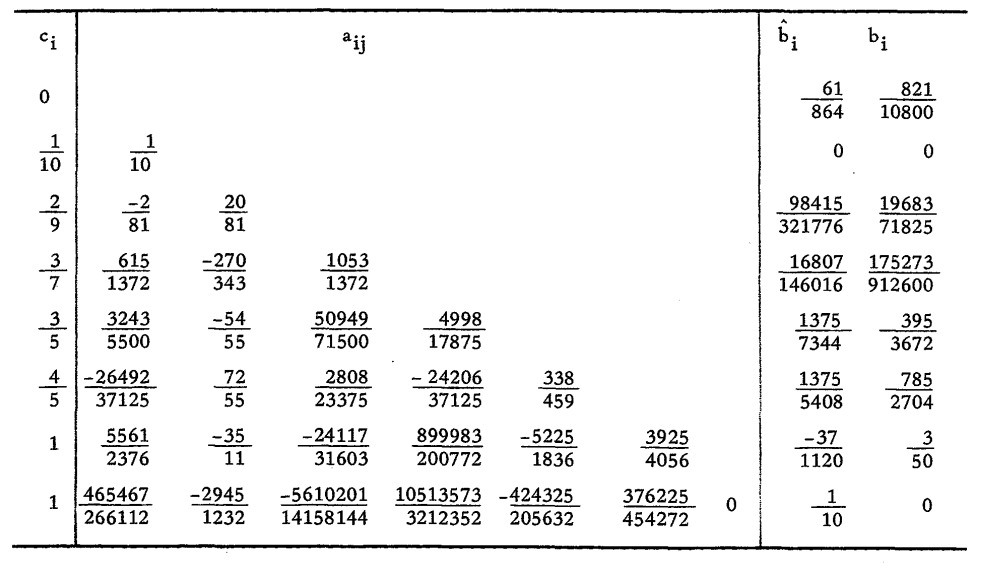
\includegraphics[width=10cm]{images/rungekutta/prdo81a}\\
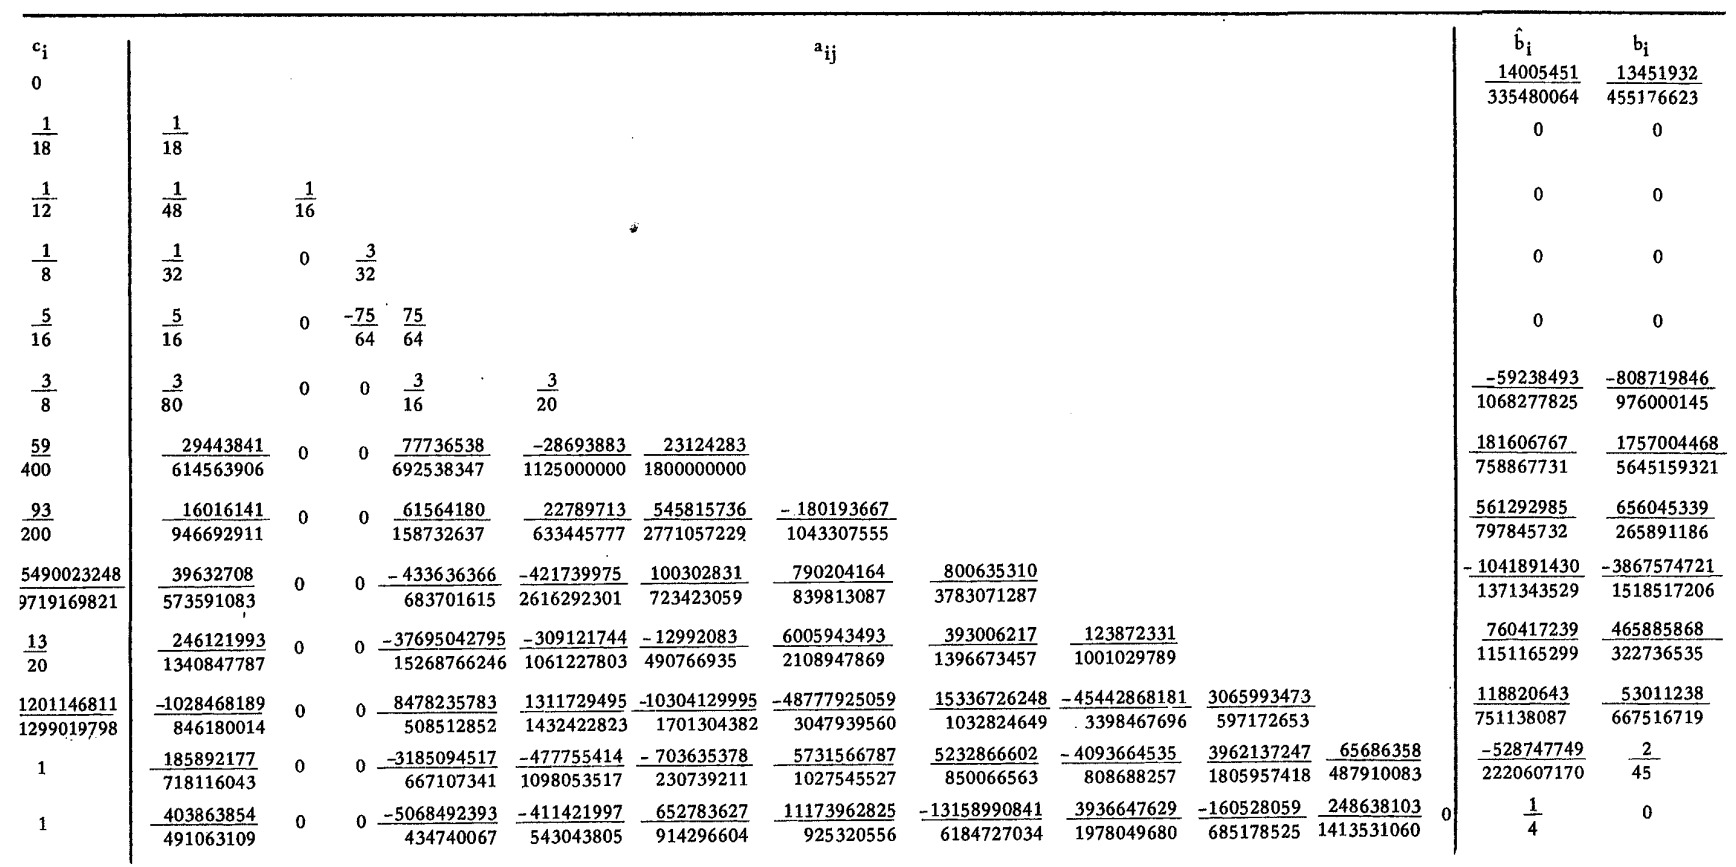
\includegraphics[width=14cm]{images/rungekutta/prdo81b}\\
{\captionfont Top: 7th order Fehlberg method; 
Middle and bottom: 6/5th and 8/7th order Dormand-Prince methods from \cite{prdo81}.}
\end{center}

\Literature:
\textcite{dopr80} (1980),
\textcite{fehl85} (1985),
\textcite{dopr86} (1986),
\textcite{caka90} (1990),
\textcite{hanw93} (1993),
\textcite{butcher03}.


%....................................................................................
\subsubsection{Using RK methods to advect particles/markers \label{sec:rkparticles}}

In the context of geodynamical modelling, one is usually faced with the following problem:
now that I have a velocity field on my FE (or FD) mesh, how can I use it to advect the Lagrangian 
markers?

Runge-Kutta methods are used to this effect but only their spatial component is used:
the velocity solution is not recomputed at the intermediate fractional timesteps, i.e. 
only the coefficients of the right hand side of the tableaus is used.

\begin{itemize}
\item The RK1 method is simple.

\begin{tabular}{c|c}
0 & \\
\hline
 & 1
\end{tabular}

\noindent Carry out a loop over markers and 
\begin{enumerate}
\item interpolate velocity $\vec\upnu_{m}$ onto each marker $m$
\item compute new position as follows: $\vec r_m(t+\delta t)=\vec r_m(t) + \vec\upnu_m \delta t$
\end{enumerate}

\item The RK2 method is also simple but requires a bit more work.

\begin{tabular}{c|cccccc}
0 & \\
1 & 1 \\
\hline
 & 1/2 & 1/2 
\end{tabular}

\noindent Carry out a loop over markers and 
\begin{enumerate}
\item interpolate velocity $\vec\upnu_{m}$ onto each marker $m$ at position $\vec r_m$
\item compute new intermediate position as follows: $\vec r_m^{(1)}(t+\delta t)=\vec r_m(t) + \vec\upnu_m \delta t/2$
\item compute velocity $\vec\upnu_{m}^{(1)}$ at position $\vec r_m^{(1)}$
\item compute new position: $\vec r_m(t+\delta t)=\vec r_m(t) + \vec\upnu_m^{(1)} \delta t$ 
\end{enumerate}
Note that the intermediate positions could be in a different element of the mesh so extra 
care must be taken when computing intermediate velocities. 

\item 
The RK3 method introduces two intermediate steps. 

\begin{tabular}{c|ccccc}
0 & \\
1/2 & {\color{chestnut} $\frac{1}{2}$ } \\
1 & {\color{violet}-1} & {\color{violet}2} \\ 
\hline
 & {\color{carrotorange} $\frac16$} & {\color{carrotorange} $\frac46$}  & {\color{carrotorange} $\frac16$}
\end{tabular}

Carry out a loop over markers and 
\begin{enumerate}
\item interpolate velocity $\vec\upnu_{m}$ onto each marker $m$ at position $\vec r_m$
\item compute new intermediate position as follows: 
$\vec r_m^{(1)}(t+\delta t)=\vec r_m(t) + {\color{chestnut} \frac{1}{2}} \vec\upnu_m \delta t$
\item compute velocity $\vec\upnu_{m}^{(1)}$ at position $\vec r_m^{(1)}$
\item compute new intermediate position as follows: 
$\vec r_m^{(2)}(t+\delta t)=\vec r_m(t) + ( {\color{violet}-1} \vec\upnu_m 
+ {\color{violet}2} \vec\upnu_m^{(1)} ) \delta t$
\item compute velocity $\vec\upnu_{m}^{(2)}$ at position $\vec r_m^{(2)}$
\item compute new position: 
$\vec r_m(t+\delta t)=\vec r_m(t) + ( 
{\color{carrotorange} \frac16} \vec\upnu_m + 
{\color{carrotorange} \frac46} \vec\upnu_m^{(1)} + 
{\color{carrotorange} \frac16} \vec\upnu_m^{(2)}    )\delta t$ 
\end{enumerate}

\end{itemize}

The following example is borrowed from \cite{maie12}, itself borrowed from Fullsack \cite[Section 5.4]{full95}.
It is a whirl flow \cite{otti89}, a flow with rotational symmetry in which concentric layers of material
rotate around  a centre with an angular velocity:
\[
\omega(r)= \omega_0 \frac{r}{r_0} \exp\left(-\frac{r}{r_0}  \right)
\]  
The box is $[-0.5,0.5]\times[-0.5,0.5]$, $r_0=0.25$, $\omega_0=0.3$ and $\delta t=1$. 
$60\times 60$ particles are regularly positioned inside the $[-0.3,0.3]\times[-0.3,0.3]$ square.
Maierova \cite{maie12} has carried out this experiment for the above Runge-Kutta methods.

\begin{center}
\includegraphics[height=4cm]{images/rk/maie12a}\\
{\captionfont Model domain with particles colored at three
different time-steps: (A) t = 0 (initial position of particles), (B) t = 50, and (C) t = 200.
The advection is computed using the fourth-order Runge-Kutta scheme. Taken from \cite{maie12}}
\end{center}

\begin{center}
\includegraphics[height=4cm]{images/rk/maie12b}
\includegraphics[height=4cm]{images/rk/maie12c}\\
{\captionfont The same plot as above, but for different advection schemes at t = 100.
Advection was computed using (A) the fourth-order Runge-Kutta scheme, (B) the mid-
point method, (C) Heun's method and (D) the explicit Euler method. Taken from \cite{maie12}}
\end{center}


 

%==============================================================================
\section{Am I in or not? - finding reduced coordinates}\label{sec:amiin}

It is quite common that at some point one must answer the question:
"Given a mesh and its connectivity on the one hand, and the coordinates of a 
point on the other, how do I accurately and quickly determine in which element 
the point resides?"

One typical occurence of such a problem is linked to the use of the Particle-In-Cell 
technique: particles are advected and move through the mesh, and need to be localised 
at every time step. This question could arise in the context of a benchmark where 
certain quantities need to be measured at specific locations inside the domain. 

%-------------------------------------------
%-------------------------------------------
\subsubsection{Two-dimensional space}

We shall first focus on quadrilaterals. There are many kinds of quadrilaterals as shown 
hereunder: 

\begin{center}
\includegraphics[width=12cm]{images/quadrilaterals} \\
{\captionfont Taken from Wikipedia 
\url{https://en.wikipedia.org/wiki/Quadrilateral#/media/File:Quadrilaterals.svg}}
\end{center}

%..................................................
\paragraph{The trivial case of rectangular elements} 

Testing whether the point $M$ is inside the element is trivial. 
For $x_0 \leq x_M \leq x_2$ and $y_0 \leq y_M \leq y_2$, its reduced coordinates
are given by
\begin{eqnarray}
r_M &=& \frac{2}{x_2-x_0}(x_M-x_0) -1 = \frac{2}{h_x}(x_M-x_0)-1  \nn\\
s_M &=& \frac{2}{y_2-y_0}(y_M-y_0) -1 = \frac{2}{h_y}(y_M-y_0)-1  
\end{eqnarray}

\begin{center}
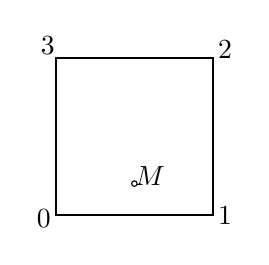
\begin{tikzpicture}
%\draw[step=0.5cm,gray,very thin] (0,0) grid (4,4); %background grid
\draw[thick] (1,1) -- (3,1) -- (3,3) -- (1,3) -- cycle;  
\node[] at (0.85,0.95) {0};
\node[] at (3.15,1) {1};
\node[] at (3.15,3.1) {2};
\node[] at (0.9,3.15) {3};
\node[] at (2.2,1.5) {$M$};
\draw (2.,1.4) circle (1pt);
\end{tikzpicture}\\
\end{center}


%..................................................
\paragraph{An intermediate case} We make the following assumption that the lateral sides of the  
element are vertical while the bottom and top are not necessarily horizontal:

\begin{center}
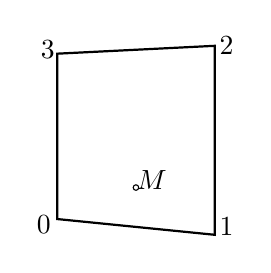
\begin{tikzpicture}
%\draw[step=0.5cm,gray,very thin] (0,0) grid (4,4); %background grid
\draw[thick] (1,1) -- (3,0.8) -- (3,3.2) -- (1,3.1) -- cycle;  
\node[] at (0.83,0.93) {0};
\node[] at (3.15,0.9) {1};
\node[] at (3.15,3.2) {2};
\node[] at (0.88,3.15) {3};
\node[] at (2.2,1.5) {$M$};
\draw (2.,1.4) circle (1pt);
\end{tikzpicture}\\
\end{center}

\noindent Because the sides are verical then if $x_0 \leq x_M \leq x_2$ then 
\[
r_M = \frac{2}{x_2-x_0}(x_M-x_0) -1 
\]
Then, if $M$ is inside the element then its $y$ coordinate is given by
\[
y_M = \sum_i \bN_i(r_M,s_M) y_i
\]
where $\bN_i$ are the four $Q_1$ basis functions associated to the vertices.
Assuming we know $r_M$ then we can solve for $s_M$:
\begin{eqnarray}
y_M &=&  
\frac{1}{4}(1-r_M)(1-s_M) y_0+
\frac{1}{4}(1+r_M)(1-s_M) y_1+
\frac{1}{4}(1+r_M)(1+s_M) y_2+
\frac{1}{4}(1-r_M)(1+s_M) y_3 \nn\\
&=& 
\frac{1}{4} \left[
(1-r)y_0+(1+r)y_1+(1+r)y_2+(1-r)y_3 +s_M [ -(1-r)y_0 - (1+r)y_1+(1+r)y_2+(1-r)y_3  ] 
\right] \nn 
\end{eqnarray}
or, 
\[
s_M = \frac{ 4y_M - [(1-r_M)y_0+(1+r_M)y_1+(1+r_M)y_2+(1-r_M)y_3]  }{ -(1-r_M)y_0 -(1+r_M)y_1+(1+r_M)y_2+(1-r_M)y_3 } 
\]
If the obtained value is in $[-1,1]$ then the point $M$ is in the element.
Verification: when $y_1=y_0$ and $y_2=y_3$ then 
\begin{eqnarray}
s_M 
&=& \frac{4 y_M - [(1-r_M)y_0+(1+r_M)y_0+(1+r_M)y_3+(1-r_M)y_3]  }{ -(1-r_M)y_0 - (1+r_M)y_0+(1+r_M)y_3+(1-r_M)y_3 } \nn\\
&=& \frac{4 y_M - [ 2 y_0 + 2 y_3]  }{ -2 y_0 + 2 y_3    }  \nn\\
&=& \frac{1}{y_3-y_0} [2 y_M - (  y_0 +  y_3) ] \nn\\ 
&=& \frac{1}{y_3-y_0} [2 y_M -  2 y_0 +y_0 -  y_3)  ] \nn\\ 
&=& \frac{2}{y_3-y_0} (y_M - y_0) - 1 
\end{eqnarray}
which is the expression that corresponds to a rectangular element as seen previously.

%..................................................
\paragraph{A generic quadrilateral}

We wish to arrive at a single algorithm which is applicable to all quadrilaterals and we now focus  
on an irregular quadrilateral (no face is parallel to the axis of the coordinate system). 

\begin{center}
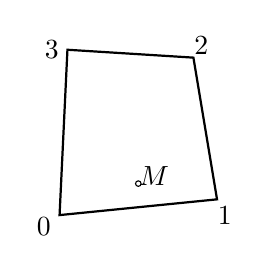
\begin{tikzpicture}
%\draw[step=0.5cm,gray,very thin] (0,0) grid (4,4); %background grid
\draw[thick] (1,1) -- (3,1.2) -- (2.7,3) -- (1.1,3.1) -- cycle;  
\node[] at (0.8,0.85) {0};
\node[] at (3.1,1) {1};
\node[] at (2.8,3.15) {2};
\node[] at (0.9,3.1) {3};
\node[] at (2.2,1.5) {$M$};
\draw (2.,1.4) circle (1pt);
\end{tikzpicture}\\
\end{center}

\noindent Several rather simple options exist:
\begin{itemize}
\item we could subdivide the quadrilateral into two triangles and check whether point $M$ is inside any of them (as it turns out, this problem is rather straightforward for triangles. Simply google it.)
\item We could check that point $M$ is always on the left side of segments $0\rightarrow 1$, $1\rightarrow 2$, $2\rightarrow 3$, $3\rightarrow 0$.
\item ...  
\end{itemize}

Any of these approaches will work although some might be faster than others. 
In three-dimensions all will however become 
cumbersome to implement and might not even work at all. 
Fortunately, there is an elegant way to answer the question, as 
detailed in the following subsection, which works both in 2D and 3D.

%-------------------------------------------
\subsubsection{Three-dimensional space}

If point $M$ is inside the quadrilateral, there exist a set of reduced 
coordinates $r,s,t\in[-1:1]^3$ such that 

\[
\sum_{i=1}^4 \bN_i(r_M,s_M,t_M) x_i = x_M
\quad\quad\quad
\sum_{i=1}^4 \bN_i(r_M,s_M,t_M) y_i = y_M
\quad\quad\quad
\sum_{i=1}^4 \bN_i(r_M,s_M,t_M) z_i = z_M
\]
This can be cast as a system of three equations and three unknowns. 
Unfortunately, each basis function $\bN_i$ 
contains a term $rst$ (as well as $rs$, $rt$, and $st$) 
so that it is not a linear system.
We must then use an iterative technique: the algorithm starts with 
a guess for values $r_M,s_M,t_M$ and 
improves on their value iteration after iteration. 
In what follows the subscript $M$ is dropped from $r,s,t$.

The classical way of solving nonlinear systems of equations is Newton's method. 
\index{general}{Newton's method}
We can rewrite the equations above as ${\bm F}(r,s,t)=0$:
\begin{eqnarray}
\sum_{i=1}^8 \bN_i(r,s,t) x_i - x_M&=&0 \nonumber\\
\sum_{i=1}^8 \bN_i(r,s,t) y_i - y_M&=&0 \nonumber\\
\sum_{i=1}^8 \bN_i(r,s,t) z_i - z_M&=&0
\end{eqnarray}
or,
\begin{eqnarray}
F_r(r,s,t)&=&0 \nonumber\\
F_s(r,s,t)&=&0 \nonumber\\
F_t(r,s,t)&=&0 \nonumber
\end{eqnarray}
so that we now have to find the zeroes of continuously differentiable 
functions ${\bm F}:\mathbb{R} \rightarrow \mathbb{R}$.
The recursion is simply:
\[
\left(
\begin{array}{c}
r_{k+1} \\s_{k+1} \\ t_{k+1}
\end{array}
\right)
=
\left(
\begin{array}{c}
r_{k} \\s_{k} \\ t_{k}
\end{array}
\right)
- J_F(r_k,s_k,t_k) ^{-1} 
\left(
\begin{array}{c}
F_r(r_k,s_k,t_k) \\
F_s(r_k,s_k,t_k)\\
F_t(r_k,s_k,t_k)
\end{array}
\right)
\]
where $J$ the Jacobian matrix:
\begin{eqnarray}
J_F(r_k,s_k,t_k)
&=&
\left(
\begin{array}{ccc}
\frac{\partial F_r}{\partial r}(r_k,s_k,t_k) & \frac{\partial F_r}{\partial s}(r_k,s_k,t_k) & \frac{\partial F_r}{\partial t}(r_k,s_k,t_k) \\\\
\frac{\partial F_s}{\partial r}(r_k,s_k,t_k) & \frac{\partial F_s}{\partial s}(r_k,s_k,t_k) & \frac{\partial F_s}{\partial t}(r_k,s_k,t_k) \\\\
\frac{\partial F_t}{\partial r}(r_k,s_k,t_k) & \frac{\partial F_t}{\partial s}(r_k,s_k,t_k) & \frac{\partial F_t}{\partial t}(r_k,s_k,t_k) 
\end{array}
\right) \nonumber\\
&=&
\left(
\begin{array}{ccc}
\sum\limits_{i=1}^8 \frac{\partial \bN_i}{\partial r}(r_k,s_k,t_k) x_i &
\sum\limits_{i=1}^8 \frac{\partial \bN_i}{\partial s}(r_k,s_k,t_k) x_i &
\sum\limits_{i=1}^8 \frac{\partial \bN_i}{\partial t}(r_k,s_k,t_k) x_i \\
\sum\limits_{i=1}^8 \frac{\partial \bN_i}{\partial r}(r_k,s_k,t_k) y_i &
\sum\limits_{i=1}^8 \frac{\partial \bN_i}{\partial s}(r_k,s_k,t_k) y_i &
\sum\limits_{i=1}^8 \frac{\partial \bN_i}{\partial t}(r_k,s_k,t_k) y_i \\
\sum\limits_{i=1}^8 \frac{\partial \bN_i}{\partial r}(r_k,s_k,t_k) z_i &
\sum\limits_{i=1}^8 \frac{\partial \bN_i}{\partial s}(r_k,s_k,t_k) z_i &
\sum\limits_{i=1}^8 \frac{\partial \bN_i}{\partial t}(r_k,s_k,t_k) z_i 
\end{array}
\right) \nonumber 
\end{eqnarray}
In practice, we solve the following system:
\[
J_F(r_k,s_k,t_k) 
\left[  
\left(
\begin{array}{c}
r_{k+1} \\s_{k+1} \\ t_{k+1}
\end{array}
\right)
-
\left(
\begin{array}{c}
r_{k} \\s_{k} \\ t_{k}
\end{array}
\right)
\right]=-
\left(
\begin{array}{c}
F_r(r_k,s_k,t_k) \\
F_s(r_k,s_k,t_k)\\
F_t(r_k,s_k,t_k)
\end{array}
\right)
\]
Finally, the algorithm goes as follows:
\begin{itemize}
\item set guess values for $r,s,t$ (typically 0)
\item loop over k=0,...
\item Compute rhs= $-{\bm F}(r_k,s_k,t_k)$ 
\item Compute matrix $J_F(r_k,s_k,t_k)$
\item solve system for $(dr_k,ds_k,dt_k)$
\item update $r_{k+1}=r_k+dr_k$, $s_{k+1}=s_k+ds_k$, $t_{k+1}=t_k+dt_k$ 
\item stop iterations when $(dr_k,ds_k,dt_k)$ is small
\item if $r_k,s_k,t_k\in[-1,1]^3$ then $M$ is inside.
\end{itemize}
This method converges quickly but involves iterations, and multiple 
solves of $3\times 3$ systems which, when carried out for each marker 
and at each time step can prove to be expensive. 
A simple modification can be added to the above algorithm: 
iterations should be carried out {\it only}
when the point $M$ is inside of a cuboid of 
size $[\min\limits_i{x_i}:\max\limits_i{x_i}]\times[\min\limits_i{y_i}:\max\limits_i{y_i} ]
\times[\min\limits_i{z_i}:\max\limits_i{z_i}]$ where the sums run over the vertices of the element. 
In 2D this translates as follows: only carry out Newton iterations when $M$ is inside the red rectangle!
\begin{center}
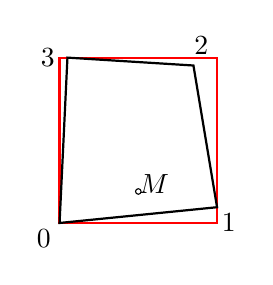
\begin{tikzpicture}
%\draw[step=0.5cm,gray,very thin] (0,0) grid (4,4); %background grid
\draw[thick,red] (1,1) -- (3,1) -- (3,3.1) -- (1,3.1) -- cycle;  
\draw[thick] (1,1) -- (3,1.2) -- (2.7,3) -- (1.1,3.1) -- cycle;  
\node[] at (0.8,0.8) {0};
\node[] at (3.15,1) {1};
\node[] at (2.8,3.25) {2};
\node[] at (0.85,3.1) {3};
\node[] at (2.2,1.5) {$M$};
\draw (2.,1.4) circle (1pt);
\end{tikzpicture}\\
\end{center}

Note that the algorithm above extends to high degree elements 
such as $Q_2$ and higher, even with curved sides.
As shown in the 2D case if the element is a cuboid or 
if all its lateral faces are vertical then one can 
compute the reduced coordinates without using an iterative method.


%-----------------------------------------------------
\subsubsection{Three-dimensional space - special case}

We assume that the mesh is such that the cross section of all $Q_1$ elements 
is a rectangle in the $xy$-plane. 

Let $(x,y,z)$ be a point inside the element. 
The global coordinates $x,y,z$ are obtained from the 
reduced coordinates $r,s,t$ via the basis the basis functions:
\begin{eqnarray}
x=\sum_{i=1}^8 \bN_i (r,s,t) x_i \qquad 
y=\sum_{i=1}^8 \bN_i (r,s,t) y_i  \qquad 
z=\sum_{i=1}^8 \bN_i (r,s,t) z_i \label{xyz}
\end{eqnarray}
Let 
\begin{eqnarray}
{\vec v}_1 &=& (+1,+1,+1,+1,+1,+1,+1,+1) \nn\\
{\vec v}_2 &=& (-1,+1,+1,-1,-1,+1,+1,-1) \nn\\
{\vec v}_3 &=& (-1,-1,+1,+1,-1,-1,+1,+1) \nn\\
{\vec v}_4 &=& (-1,-1,-1,-1,+1,+1,+1,+1) \nn\\
{\vec v}_5 &=& (+1,-1,+1,-1,+1,-1,+1,-1) \nn\\
{\vec v}_6 &=& (+1,-1,-1,+1,-1,+1,+1,-1) \nn\\
{\vec v}_7 &=& (+1,+1,-1,-1,-1,-1,+1,+1) \nn
\end{eqnarray}
and 
\begin{eqnarray}
{\vec x} &=& (x_1,x_2,x_3,x_4,x_5,x_6,x_7,x_8) \nn\\
{\vec y} &=& (y_1,y_2,y_3,y_4,y_5,y_6,y_7,y_8) \nn\\
{\vec z} &=& (z_1,z_2,z_3,z_4,z_5,z_6,z_7,z_8) \nn
\end{eqnarray}
then Eqs.~\eqref{xyz} can also be written
\begin{eqnarray}
x&=&\frac{1}{8} \left( {\vec v}_1 + r  {\vec v}_2 + s  {\vec v}_3 + t  {\vec v}_4 
                 + rs  {\vec v}_5 + rt {\vec v}_6 + st {\vec v}_7 \right) \cdot {\vec x} \nn\\ 
y&=&\frac{1}{8} \left( {\vec v}_1 + r  {\vec v}_2 + s  {\vec v}_3 + t  {\vec v}_4 
                 + rs  {\vec v}_5 + rt {\vec v}_6 + st {\vec v}_7 \right) \cdot {\vec y} \nn\\
z&=&\frac{1}{8} \left( {\vec v}_1 + r  {\vec v}_2 + s  {\vec v}_3 + t  {\vec v}_4 
                 + rs  {\vec v}_5 + rt {\vec v}_6 + st {\vec v}_7 \right) \cdot {\vec z} \label{zzz}
\end{eqnarray}
If the element has a rectangular cross-section $s_x \times s_y$ then 
\begin{eqnarray}
{\vec x} &=& (x_0,x_0+s_x,x_0+s_x,x_0,x_0,x_0+s_x,x_0+s_x,x_0) \nn\\
{\vec y} &=& (y_0,y_0,y_0+s_y,y_0+s_y,y_0,y_0,y_0+s_y,y_0+s_y) \nn
\end{eqnarray}
which yields
\begin{eqnarray}
r&=& 2\frac{x-x_0}{s_x}-1  \nn\\
s&=& 2\frac{y-y_0}{s_y}-1  \nn
\end{eqnarray}
Since the local coordinates $r$ and $s$ can be easily computed, one can use Eq.~\eqref{zzz} to obtain $t$:
\[
t=\frac{8z - ({\vec v}_1 + r {\vec v}_2 + s {\vec v}_3 + rs  {\vec v}_5 ) \cdot {\vec z}} 
{ ({\vec v}_4  + r  {\vec v}_6 + s  {\vec v}_7)  \cdot {\vec z} }
\]







 
